% !TeX program = lualatex
% !TeX root = luaking.tex
% !TeX encoding = UTF-8
% !TeX spellcheck = cs_CZ
%---------------------------------------------------------------------------------------------------
\graphicspath{{../src/MAI/img/}}
% file mai1ch04b.tex
%---------------------------------------------------------------------------------------------------
\setchaptertoc
\chapter{Náhodné veličiny}\label{mai:IchapIVb}
  \epigraph{\emph{The true logic of this world is in the calculus of probabilities.}}{James Clerk 
    Maxwell}
  \section{Úvod}\label{mai:IchapIVsecIII}
    Hodnota některých veličin je určena jednoznačně a „jednou provždy“. Kdykoli budeme její hodnotu 
    zjišťovat, tehdy dostaneme totéž - takže ji ani opakovaně zjišťovat nemusíme. Příkladem může 
    být skoro prázdná peněženka, ve které jsou třeba tři koruny. Dokud nebudeme pracovat a do 
    peněženky něco nepřidáme, bude hodnota veličiny \(X\) (počet korun v peněžence) stále rovna 
    \num{3}. Nemá smysl se do peněženky vůbec dívat. Pokud budeme do peněženky přidávat každý den 
    dvě koruny, také budeme vědět, jak se veličina \(X\) mění, aniž bychom se do peněženky dívali. 
    Po \(n\) dnech bude hodnota \(X = 3 + 2n\). Většina veličin, se kterými se setkáváme, se však 
    takto nechová. Jejich hodnoty se totiž často řídí náhodnými vlivy, takže při každém
    měření veličiny \(X\), tj. zjišťování její hodnoty, můžeme získat odlišný výsledek než při 
    měřeních předchozích. Uveďme některé příklady náhodných veličin.
    
    \begin{itemize}
      \item \textbf{Příklad s novorozenci}: Nechť jé veličinou \(X\) počet chlapců ve stovce 
            novorozených dětí. Zkušenost říká, že tento počet je v průměru o něco větší než 
            \num{50}, avšak pro různé skupiny po stovce novorozených dětí bude počet chlapců 
            kolísat. V jedné skupině bude \num{52}, v jiné \num{54}, někde třeba \num{60}, nebo 
            také \num{45}.
      \item \textbf{Příklad s meteoroidy a meteority}: Pro astronomy může být důležitou veličinou 
            \(X\) počet meteoroidů, které za rok dopadnou do zemské atmosféry. Jinou veličinou, 
            třeba \(K\), může být roční počet meteoritů, tj. těch meteoroidů, které v atmosféře 
            neshořely zcela, ale jejich část dopadla na povrch Země. Také tyto hodnoty budou pro 
            každý roční interval poněkud odlišné, neboť i počet dopadnuvších meteoroidů a 
            meteoritů podléhá vlivům, které se nedají přesně předvídat.
      \item \textbf{ Příklad s tlakoměrem}: Bude-li lékař měřit pacientovi tlak několikrát po 
            sobě, určitě také naměří několik různých hodnot. Krevní tlak je citlivý na náhodné 
            vlivy, třeba i na vnitřní rozrušení pacienta vyplývající ze strachu z bílého pláště.
      \item \textbf{Opakovaná měření fyzikální veličiny}: Chceme-li změřit třeba odpor elektrického
            vodiče (drátu), jedná se o měření nepřímé. Nemůžeme odpor změřit přímo, třeba jako      
            to můžeme udělat pro délku. Většinou měříme napětí \(U\) na vodiči a proud \(I\), který 
            jím protéká. Odpor pak zjišťujeme jako podíl \(R = U/I\). Změříme-li napětí i proud 
            jednou, dostaneme konkrétní hodnotu \(R\). Budeme-li měření napětí a proudu provádět 
            opakovaně, budeme dostávat poněkud odlišné hodnoty \(U\) a \(I\), a tedy i odlišné 
            hodnoty \(R\). Sledované veličiny se chovají jako náhodné. Je to způsobeno řadou 
            náhodných vlivů jak na veličiny samotné, tak na jejich měření (nepřesnost odečítání 
            údajů na stupnicích, apod.).
    \end{itemize}
  
    Při každém fyzikálním (a vlastně i nefyzikálním) experimentu máme co do činění s náhodnými 
    veličinami. Při chemických analýzách je náhodnou veličinou třeba koncentrace dané látky
    v roztoku, při experimentech biologických třeba počet uhynuvších rostlin ve stovce sazenic, 
    počet pozorovaných prvoků v zorném poli mikroskopu, výskyt vzácných ptáků ve sledované 
    lokalitě, apod. V následujících odstavcích definujeme náhodné veličiny přesněji a naučíme se s 
    nimi zacházet. Uvidíme, že zjištění určité hodnoty náhodné veličiny je otázkou jisté 
    pravděpodobnosti. Také lépe objasníme, co znamená vyjádření „v průměru“, které jsme občas v 
    předchozím textu použili a intuitivně mu jistě rozuměli.
  
    \subsection{Jak dobrý je to střelec - diskrétní rozdělení}
      Mimořádně vhodnou ukázkou náhodné veličiny je příklad se sportovním střelcem, kterým jsme
      uvedli celou kapitolu o pravděpodobnostech.
  
      %--Ještě jednou střelba, tentokrát přesněji---------------------
      % !TeX spellcheck = cs_CZ
\begin{mdframed}[style=mdexam]
  \begin{example}\label{mai:exam064}
    \textbf{Ještě jednou střelba, tentokrát přesněji}\newline
    Názvem pochopitelně nemyslíme přesnější střelbu, ale přesnější komentář, který již bude založen
    na našich znalostech o pravděpodobnosti. Dejme tomu, že podmínky střelby jsou pevně dány a
    nemění se. Patří k nim zcela jistě typ zbraně, typ terče, vzdálenost stanoviště střelce od
    terče, základní povětrnostní podmínky. Výsledky jsou pak závislé na zručnosti střelce, avšak
    jsou ovlivněny náhodným i vlivy (foukne nenadálý vítr, střelec se lekne, zatřese se mu ruka,
    náhodně se mírně pozmění vzdálenost ústí hlavně od terče nebo její sklon, apod.). Počty
    dosažených bodů daného střelce při jednom výstřelu, nebo při sérii deseti výstřelů, atd., jsou
    tedy náhodnými veličinami. Pokusme se posoudit zručnost střelce přesněji. Označme jako náhodnou
    veličinu \(X\) počet bodů dosažených při jednom výstřelu. Nejprve určeme, jakých hodnot může
    nabývat. Všichni víme, jak vypadá běžný střelecký terč. Aby však naše počty nebyly příliš
    komplikované a zdlouhavé, uvažujme o terči mnohem jednodušším. Bude tvořen vnitřním černým
    kruhem s hodnotou \(3\) body, dále středním šedivým mezikružím s hodnotou \(2\) body a vnějším
    bílým mezikružím s hodnotou \(1\) bod. Střelba do terče mimo vnější kružnici nebo zcela mimo
    terč představuje bodovou hodnotu \(0\). Při jednom výstřelu tedy může střelec docílit v principu
    jakékoli z možných hodnot

    {\centering
      \captionsetup{type=figure}
      \luafigure[0.6]{mai_fig070.pdf}
      \captionof{figure}{Ilustrace k příkladu \ref{mai:exam064}}
      \label{mai:fig070}
    \par}
    \vspace{0.5em}
    \begin{equation*}
      X\in\{x_1, x_2, x_3,x_4\} = \{0,1,2,3\}.
    \end{equation*}
    Informace, jakých hodnot může náhodná veličina nabývat, je jistě nejen cenná, ale je pro
    jakékoli další úvahy nezbytná. Sama o sobě je však nepostačující. O střelcově zručnosti se na
    základě konstrukce terče nic nedovídáme. Kvalitativně jinou informaci získáme, víme-li, že
    možných hodnot zásahu dociluje střelec s následujícími pravděpodobnostmi:

    {\centering
      \begin{tabular}{c|rrrr}
        \(x_i\)    &      0     &      1     &      2     &      3       \\
        \hline
        \(p_i\)    & \num{0.03} & \num{0.28} & \num{0.52} & \num{0.17} 
      \end{tabular}
    \par}

    Můžeme tak třeba zjistit, kolika bodů střelec zhruba docílí s vysokou pravděpodobností při pěti
    výstřelech. Tento počet je
    \begin{gather*}
      5\cdot(\num{0.03}\cdot0 + \num{0.28}\cdot1 + \num{0.52}\cdot2 + \num{0.17}\cdot3) = 
      5\cdot\num{1.83} = \num{9.15} \simeq 9.
    \end{gather*}
    Pro každou pětici výstřelů může být počet dosažených bodů samozřejmě poněkud odlišný. Veličina
    \(Y\) představující počet dosažených bodů na pět výstřelů je rovněž veličinou náhodnou. Je nám
    však jasné, že hodnota dosažených bodů v každé pětici výstřelů je s vysokou pravděpodobností
    blízká číslu 9. Co to znamená „s vysokou pravděpodobností“? Dokážeme ji spočítat? Pokusme se o
    to. Především bychom museli určit, o kolik bodů se smí dosažený počet lišit od hodnoty 9,
    abychom jej ještě považovali za „blízký číslu 9“ . Tato volba závisí čistě na naší vůli a bude
    jí odpovídat i vypočtená pravděpodobnost. Dejme tomu, že zvolíme tento interval od 7 do 11 bodů
    včetně. Jev, jehož pravděpodobnost hledáme, je tedy
    \begin{itemize}
      \item \(A\) : Při pěti výstřelech získá střelec \num{7} nebo \num{8} nebo \num{9} nebo \num{10} 
            nebo \num{11} bodů.
      \item[] Jevy
      \item \(A_j\) : Střelec získá při pěti výstřelech \(j\) bodů.
    \end{itemize}
    jsou po dvou neslučitelné, pravděpodobnost jevu \(A\) tedy bude rovna součtu pravděpodobností
    \begin{equation*}
      p(A) = \sum_{j=7}^{11} p(A_j).
    \end{equation*}
   
    Pozor! Pravděpodobnosti \(p(Aj)\) jsou odlišné od pravděpodobností zadaných v první tabulce. Ta
    se totiž týká pěti výstřelů, zatímco tabulka \ref{mai:tab004} je pro jeden výstřel. Musíme tedy
    určit pravděpodobnosti \(p(A_j)\). K tomu je třeba zjistit všechny možnosti, jak docílit součtu
    bodů \(j\) pomocí pěti sčítanců nabývajících hodnot \num{0} až \num{3}. Soupis je v následující
    tabulce. Tabulka uvádí různé rozklady součtu na sčítance, počet případů, jak se tento rozklad
    realizuje (různé pořadí dosažených bodů při jednotlivých výstřelech) a pravděpodobnosti
    jednotlivých rozkladů zaokrouhlené na tři platná místa.

    Jak jsme spočítali pravděpodobnosti jednotlivých rozkladů? Dejme tomu, že počet bodů dosažených
    při pěti výstřelech je \(j\). Nechť \(j = j_1 + j_2 + j_3 + j_4 + j_5\) je rozklad hodnoty \(j\)
    na součet pěti sčítanců. Čísla \(j_1\) až \(j_5\) se pohybují od \num{0} do \num{3}, mohou být i
    shodná. Například jeden z možných rozkladů bodového součtu \(j = 9\) je \(9 = 3 + 2 + 2 + 1 +
    1\). Pravděpodobnost, že při pěti nezávislých výstřelech budou jednotlivé zásahy činit \(j_1\),
    \(j_2\), \(j_3\) , \(j_4\)a \(j_5\) bodů, je
    \begin{equation*}
      p_{j1}p_{j2}p_{j3}p_{j4}p_{j5}.
    \end{equation*}
    Pro případ zvoleného konkrétního rozkladu čísla \num{9} je to \(p_3p_2^2p_1^2\) - Zásahy s
    bodovým ziskem \(j_1\) až \(j_5\) mohou být realizovány v různých pořadích (například \(\num{3}
    + \num{2} + \num{2} + \num{1} + \num{1} = \num{2} + \num{3} + \num{2} + \num{1} + \num{1}
    =\ldots\), atd.). Označme počet všech takových pořadí \(n_{j_1\ldots j_5}\). (Pro \(j = \num{3}
    + \num{2} + \num{2} + \num{1} + \num{1}\) je \(n_{32211} = \binom{5}{2}\binom{3}{2} = 30\): Dvě
    z pěti pozic pro umístění dvou dvojek lze vybrat \(\binom{5}{2}\) způsoby, ze zbývajících tří
    pozic lze dvě pro umístění jedniček vybrat \(\binom{3}{2}\) způsoby a na trojku zbude poslední
    pozice.) Pravděpodobnost \(p_{j_1\ldots j_5}\) daného rozkladu čísla \(s\) pak je
    \begin{equation*}
      p_{j_1\ldots j_5} = n_{j_1\ldots j_5}p_{j_1}p_{j_2}p_{j_3}p_{j_4}p_{j_5}
    \end{equation*}

    {\centering
    \resizebox{1\textwidth}{!}{%
    \begin{tabular}{c|rrrr}
      součet \(j\)& sčítance   &    počet   & ppst rozkladu & \(p(A_j)\) \\ \hline
            7     & 3+3+1+0+0  & \num{30}   & \num{2.18e-4} & \num{0.102} \\
                  & 3+2+2+0+0  & \num{30}   & \num{1.24e-3} & \\
                  & 3+2+1+1+0  & \num{60}   & \num{1.25e-2} & \\
                  & 3+1+1+1+1  & \num{5}    & \num{5.22e-3} & \\
                  & 2+2+2+1+0  & \num{20}   & \num{2.36e-2} & \\
                  & 2+2+1+1+1  & \num{10}   & \num{5.94e-2} & \\ \hline
            8     & 3+3+2+0+0  & \num{30}   & \num{4.06e-4} & \num{0.185} \\
                  & 3+3+1+1+0  & \num{30}   & \num{2.04e-3} & \\
                  & 3+2+2+1+0  & \num{60}   & \num{2.32e-2} & \\
                  & 3+2+1+1+1  & \num{20}   & \num{3.88e-2} & \\
                  & 2+2+2+2+0  & \num{5}    & \num{1.10e-2} & \\
                  & 2+2+2+1+1  & \num{10}   & \num{1.10e-1} & \\ \hline
            9     & 3+3+3+0+0  & \num{10}   & \num{4.42e-5} & \num{0.238} \\
                  & 3+3+2+1+0  & \num{60}   & \num{7.57e-3} & \\
                  & 3+3+1+1+1  & \num{10}   & \num{6.34e-3} & \\
                  & 3+2+2+2+0  & \num{20}   & \num{1.43e-2} & \\
                  & 3+2+2+1+1  & \num{30}   & \num{1.08e-1} & \\
                  & 2+2+2+2+1  & \num{5}    & \num{1.02e-1} & \\ \hline
          10      & 3+3+3+1+0  & \num{20}   & \num{8.25e-4} & \num{0.215} \\
                  & 3+3+2+2+0  & \num{30}   & \num{7.03e-3} & \\
                  & 3+3+2+1+1  & \num{30}   & \num{3.53e-2} & \\
                  & 3+2+2+2+1  & \num{20}   & \num{1.34e-1} & \\
                  & 2+2+2+2+2  & \num{1}    & \num{3.80e-2} & \\ \hline
          11      & 3+3+3+2+0  & \num{20}   & \num{1.53e-3} & \num{0.133} \\
                  & 3+3+3+1+1  & \num{10}   & \num{3.85e-3} & \\
                  & 3+3+2+2+1  & \num{30}   & \num{6.56e-2} & \\
                  & 3+2+2+2+2  & \num{5}    & \num{6.21e-2} & \\ \hline
    \end{tabular}}
    \captionsetup{type=table} 
    \captionof{table}{Tabulka rozkladů pro daný součet bodů: ve sloupci \uv{počet} je uveden počet 
                      kombinací, které vedou ke stejnému nástřelu (sloupec \uv{součet}) a s daným
                      bodovým ohodnocením (sloupec \uv{sčítanec})}
    \label{mai:tab004}
    \par}
    \vspace{\baselineskip}

    Pro rozklad \(\num{9} = \num{3} + \num{2} + \num{2} + \num{1} + \num{1}\) je (výsledek viz také
    v tabulce)
    \begin{equation*}
      p_{32211} =30\cdot p_3p_2^2p_1^2 = \num{30}\cdot\num{0.17}\cdot\num{0.52}^2\cdot\num{0,282} 
                \simeq \num{0.108}.
    \end{equation*}
    Pravděpodobnost \(p(A_j)\) je součtem pravděpodobností jednotlivých rozkladů čísla \(j\).
    Konečně pravděpodobnost, že střelec dosáhne bodového výsledku \(y \in [7, 11]\), je rovna součtu
    pravděpodobností \(p(A_j)\) pro \(j = 7, 8, 9, 10, 11\). Tato hodnota je \num{0.873}, tedy
    opravdu poměrně vysoká, jak jsme očekávali. Také bychom mohli říci, že střelec dosahuje při
    každé pětici výstřelů „v průměru“ \num{9} bodů, a tedy při jednom výstřelu „v průměru“ \num{1.8}
    bodů. Pokud bychom „průměrnou hodnotu“ jednoho výstřelu počítali i pro jiný počet výstřelů než
    pro pět, budeme dostávat čísla, která budou hodnotě \num{1.8} velmi blízká.
  \end{example}
\end{mdframed}
      %---------------------------------------------------------------
    
    Položme si ještě otázku, jak můžeme zjistit pravděpodobnosti, se kterými střelec dosáhne při
    jednom výstřelu daného počtu bodů. Prakticky to lze provést jedině tak, že střelec mnohokrát
    vystřelí na terč a jeho zásahy budou při tom zaznamenávány. Dejme tomu, že vystřelil \(n\)-krát 
    a že počet výstřelů, při nichž byl bodový zisk \(j\) bodů ( \(j = 0, 1, 2, 3\)), byl \(n_j\). 
    Pak pro pravděpodobnost bodového zisku \(j\) bodů při jednom výstřelu je \(p_j = n_j/n\). 
    Kdybychom provedli skutečný experiment se střelcem a počítali pravděpodobnosti \(p_j\) znovu a 
    znovu po každém dalším výstřelu, viděli bychom, že pro malé hodnoty \(n\) nejprve kolísají a 
    pro rostoucí \(n\) se začínají ustalovat a již kolísají velmi málo. Tímto postupem bychom je 
    mohli určit tak, aby byly pro náš účel rozumně přesné - třeba s přesností na dvě platná místa. 
    Rozumnou přesností je zde myšlena skutečnost, že nemá smysl chtít zjišťovat pravděpodobnost 
    třeba na šest platných míst. Vzhledem k principiální přítomnosti náhodných vlivů se kolísání 
    pravděpodobností nikdy nezbavíme, takže platná místa na pozicích, kde se kolísání trvale 
    projevuje již bez ohledu na zvyšující se \(n\), nemají smysl.
    
    V příkladu \ref{mai:exam064} jsme se již velmi těsně přiblížili důležitým charakteristikám, 
    které určují náhodnou veličinu a jsou přitom matematicky korektně definovány. Viděli jsme, že 
    známe-li jen hodnoty, kterých může náhodná veličina nabývat, nemůžeme o ní říci již nic 
    dalšího. Známe-li však ještě pravděpodobnosti, se kterými jednotlivých hodnot nabývá, můžeme o 
    ní získat již velmi mnoho informací.

    \begin{mdframed}[style=highlight]
      \textbf{Náhodnou veličinou s diskrétním rozdělením} nazýváme takovou veličinu \(X\), která
      může nabývat konečně mnoha různých hodnot \((x_1, x_2, \ldots, x_k)\) s pravděpodobnostní
      \((p_1, p_2, \ldots, p_k)\) popřípadě spočetně mnoha hodnot \((x_1, x_2, \ldots)\) s 
      pravděpodobnostmi \((p_1, p_2, \ldots)\).
    \end{mdframed}

    Jevy \(A_j\) \uv{veličina \(X\) nabývá hodnoty \(x_j\)}, jsou po dvou neslučitelné. Platí
    \begin{equation*}
      \sum_{j=1}^{k}p_j = 1, \qquad\text{resp.}\qquad \sum_{j=1}^{k=\infty}p_j = 1
    \end{equation*}
    Pokud jde o druhý z obou případů, nebudeme se jím prozatím zabývat. Soubor všech dvojic
    \begin{equation*}
      \left\lbrace(x_j, p_j)\right\rbrace,\qquad j = 1, 2, \ldots, k,
    \end{equation*}
    se nazývá \textbf{rozdělení} náhodné veličiny \(X\). Můžeme je znázornit i graficky.

    %--Bernoulliovo (binomické) rozdělení---------------------------
    % !TeX spellcheck = cs_CZ
\begin{mdframed}[style=mdexam]
  \begin{example}\label{mai:exam065}
    \textbf{Bernoulliovo (binomické) rozdělení}\newline
    Představme si opět Bernoulliův pokus o \(n\) opakováních a pravděpodobností zdaru při jednom
    opakování rovnou \(p\) (kapitola \ref{mai:IchapIVsecIIssecIV}). Náhodnou veličinu \(X\)
    definujme jako počet zdarů při tomto pokusu. Tato veličina nabývá všech celočíselných hodnot
    \(x_j = j, 0 \leq j \leq n\), přitom hodnoty \(j\) nabývá s pravděpodobností určenou vztahem
    (\ref{mai:eq055}), v němž za \(x\) dosadíme \(j\). 
    
    {\centering
      \captionsetup{type=figure}
      \luafigure[1]{mai_fig044.pdf}
      \captionof{figure}{Bernoulliovo rozdělení
      \cite[s.~229]{Musilova2009MA1}
      \label{mai:fig044}}
    \par}
    
    Získané rozdělení je tedy
    \begin{equation*}
      \lbrace j,p_j\rbrace, \quad\text{kde}\quad p_j = \binom{n}{j}p^j(1 - p)^{n-j}.
    \end{equation*}
    Graf Bernoulliova rozdělení, které je často nazýváno také binomickým, je na obrázku 
    \ref{mai:fig044} pro \(n = 15\) a \(p = 1/2\) (červený asterisk).
    
    Z grafu je názorně vidět, co to znamená, že některé hodnoty veličiny \(X\) jsou více a jiné méně 
    pravděpodobné. Hodnota \(x_i\), veličiny \(X\), které odpovídá největší pravděpodobnost \(p_i\), 
    se nazývá nejpravděpodobnější hodnota. V případě Bernoulliova rozdělení na obrázku 
    \ref{mai:fig044} jsou takové hodnoty dvě, konkrétně \(x_7 = 7\) a \(x_8 = 8\).
    
      \begin{lstlisting}[style=luaCPPStyle, caption={PPST001.m}]
        citatel= factorial(n);
        jmenovatel= factorial(n-j).*factorial(j);
        binom = citatel./jmenovatel;
        f = binom.*p.^j.*(1-p).^(n-j);
      \end{lstlisting}
  \end{example}
\end{mdframed}
    %---------------------------------------------------------------
    
    Nyní definujeme další charakteristiky náhodné veličiny. Těmi základními jsou, kromě již 
    definované \emph{nejpravděpodobnější hodnoty}, ještě \textbf{střední hodnota}, \textbf{rozptyl} 
    (popřípadě jeho odmocnina, zvaná \textbf{střední kvadratická} nebo \textbf{směrodatná 
    odchylka}), \textbf{medián}, popřípadě \textbf{P-kvantil}. Pojem střední hodnoty jsme již v 
    podstatě vybudovali v příkladu se střelcem. Nyní postup zobecníme. Předpokládejme, že při 
    velkém počtu \(n\) měření náhodné veličiny \(X\) naměříme různé hodnoty \((x_1, x_2, \ldots, 
    x_k)\) tak, že hodnota \(x_1\) byla naměřena \(n_1\)-krát, hodnota \(x_2\) \(n_2\)-krát, atd., 
    až hodnota \(x_k\) \(n_k\)-krát. Je zřejmé, že součet četností \(n_1\), \(n_2\), až \(n_k\) 
    jednotlivých hodnot musí být roven celkovému počtu měření \(n\) a že podíly
    \begin{equation*}
      p_1 = \dfrac{n_1}{n}, \qquad p_2 = \dfrac{n_2}{n}, \qquad \ldots, \qquad p_k = \dfrac{n_k}{n},
    \end{equation*}
    představují pravděpodobnosti jednotlivých hodnot veličiny \(X\). Tím je zadáno její rozdělení,
    které ji plně charakterizuje. Položme si však otázku, zda by se veličina \(X\) přece jen nedala
    charakterizovat jedinou hodnotou, která by všechny různě pravděpodobné hodnoty v jistém
    smyslu „zastupovala“. Kdybychom třeba takto měřili délku stolu, jistě bychom na otázku „Kolik
    měří stůl?“ neodpovídali tím, že bychom tazateli předložili získané rozdělení, i když by taková
    odpověď byla nejvýstižnější. Určitě bychom uvedli jedinou hodnotu. Ale jakou? I laika napadne,
    že by takovou reprezentativní hodnotou mohl být aritmetický průměr naměřených hodnot \(x_1\) až
    \(x_k\). Bylo by ale správné vzít jen prostý aritmetický průměr těchto různých hodnot a nebrat 
    ohled na skutečnost, že některé byly naměřeny s větší a jiné s menší četností? Nikoliv. 
    Reprezentativní hodnota veličiny \(X\) nemá zastupovat jen naměřené hodnoty, ale celé 
    rozdělení. Určitá hodnota \(x_j\) bude mít tím větší vliv na reprezentativní hodnotu, s čím 
    větší četností byla naměřena. Protože byla naměřena \(n_j\)-krát, musíme ji také tolikrát do 
    aritmetického průměru započíst.Získáváme tak \textbf{vážený aritmetický průměr} naměřených 
    hodnot, neboli \emph{střední hodnotu}
    
    \begin{mdframed}[style=highlight]
      \begin{align}\label{mai:eq059}
        \left\langle x \right\rangle 
          &= \dfrac{n_1x_1 + n_2x_2 + \cdots + n_kx_k}{n}  \nonumber \\
          &= p_1x_1 + p_2x_2 + \cdots + p_kx_k             \nonumber \\
          &= \sum_{j=1}^{k}p_jx_j.
      \end{align}
    \end{mdframed}
    Součet všech pravděpodobností \(p_1 + p_2 + \cdots + p_k\) je pochopitelně \textbf{roven jedné}.

    %--Střední hodnota Bernoulliova rozdělení-----------------------
    % !TeX spellcheck = cs_CZ
\begin{mdframed}[style=mdexam]
  \begin{example}\label{mai:exam066}
    \textbf{Bernoulliovo (binomické) rozdělení}\newline
    Pro střední hodnotu Bernoulliova rozdělení platí
    \begin{equation*}
      \langle j \rangle = \sum_{j=0}^{n}j\cdot p_j
        = \sum_{j=1}^{n}j\begin{pmatrix} n \\ j \end{pmatrix}p^j(1-p)^{n-j} = np.
    \end{equation*}
    
    Tento vztah lze dokázat matematickou indukcí vzhledem k proměnné \(n\). Na tomto místě nebudeme
    důkaz provádět pro jeho poměrnou zdlouhavost. Každý jej však může zvládnout. Vzpomeňme si v tuto
    chvíli na náš chybný intuitivní odhad v kapitole \ref{mai:IchapIVsecIIssecIV}, v níž jsme
    poprvé hovořili o Bernoulliově pokusu v souvislosti s hody mincí. Chybně jsme tam odhadli
    pravděpodobnost, že při \(n\) opakováních pokusu nastane v polovině z nich zdar. Tato chyba
    vznikla v důsledku naší zkušenosti, že když budeme mincí vícekrát házet, padne hlava (zdar)
    skutečně zhruba v polovině případů. Vidíme nyní, že \(n/2\) reprezentuje střední hodnotu náhodné
    veličiny \(X =\) \textbf{počet zdarů při \(n\) hodech mincí}. A to naší zkušenosti již odpovídá.
  \end{example}
\end{mdframed}
    %---------------------------------------------------------------
    
    Posuďme nyní situaci, kdy náhodná veličina \(Y\) je funkcí náhodné veličiny \(X, Y = f(X)\).
    V takovém případě má rozdělení veličiny \(Y\) tvar
    \begin{equation*}
      \left\lbrace (f(x_j), p_j)\right\rbrace, \qquad j = 1, 2, \ldots, k.
    \end{equation*}
    Pravděpodobnost hodnoty \(f(x_j)\) je stejná jako pravděpodobnost hodnoty \(x_j\). Pro výpočet
    střední hodnoty veličiny \(Y\) pak platí
    \begin{equation}\label{mai:eq060}
      \left\langle y \right\rangle = \sum_{j=1}^{k}f(x_j)p_j.
    \end{equation}
    (V obecnější situaci může být náhodná veličina \(Y\) funkcí několika náhodných veličin \(X_1\), 
    \(X_2\), až \(X_s\)).
    
    Může vzniknout oprávněná otázka, zda při výpočtu \(\left\langle y \right\rangle\), popřípadě 
    dalších charakteristik veličiny \(Y\), nevznikne nějaký problém, nebude-li funkce \(f(X)\) 
    prostá. V takovém případě by totiž některé hodnoty veličiny \(Y\) splynuly i pro různá \(x_j\). 
    Například pro \(Y = f(X) = X^2\) by pro hodnoty \(x_r\) a \(x_s\) vázané vztahem \(x_r = -x_s\) 
    (pokud by veličina \(X\) směla takových hodnot nabývat) platilo \(y_{rs} = y_r = y_s\). 
    Pravděpodobnost této společné hodnoty by pak přece byla \((p_r + p_s)\). Tato úvaha je 
    samozřejmě správná, avšak ve výpočtu střední hodnoty veličiny Y
    podle vztahu (\ref{mai:eq060}) je již obsažena. Do součtu totiž vstupují sčítance \(y_rp_r\) i 
    \(y_sp_s\), jejichž součet je při rovnosti \(y_r = y_s\) roven \(y_{rs}(p_r +p_s)\) Společná 
    hodnota \(y_{rs}\) je tedy započtena se správnou vahou.
    
    Uvažujme nyní o tom, jak „směrodatná“, tj. do jaké míry opravdu „reprezentativní“, je
    střední hodnota náhodné veličiny. Intuitivně cítíme, že střední hodnota bude reprezentovat
    rozdělení náhodné veličiny tím lépe, čím méně se od ní budou jednotlivé hodnoty odchylovat na 
    obě strany. Význam slova „odchylovat“ musíme ovšem nějak kvantitativně zachytit.
    \emph{Odchylkou} hodnoty \(x_j\) veličiny \(X\) od střední hodnoty \(\left\langle x 
    \right\rangle\) budeme celkem přirozeně rozumět rozdíl \((x_j - \langle x\rangle)\). Vzniká tak 
    náhodná veličina \(\Sigma = X - \langle x \rangle\) s rozdělením \(\{(x_j - \langle x\rangle, 
    p_j)\}\), \(j = 1, 2, \ldots, k\) . Bude tou správnou charakteristikou odchýlení hodnot 
    veličiny \(X\) od střední hodnoty střední hodnota \(\langle\sigma\rangle\)? Vypočtěme ji 
    (odhadněte předem, co asi tak vyjde):
    \begin{align*}
      \langle\sigma\rangle 
          &= \sum_{j=1}^{k}(x_j - \langle x\rangle)p_j
           = \sum_{j=1}^{k}x_jp_j - \langle x\rangle\sum_{j=1}^{k}p_j   \\
          &= \langle x\rangle - \langle x\rangle = 0.
    \end{align*}
    Čekali jste to? Nepochybně ano. Veličina \(X - \langle x\rangle\) nedává tedy žádný obraz o 
    tom, jak jsou hodnoty \(x_j\) „rozptýleny“ okolo střední hodnoty \(\langle x\rangle\). Kladné 
    odchylky jsou to tiž kompenzovány těmi zápornými. Aby k takové kompenzaci nedošlo, stačí vzít 
    v úvahu absolutní hodnotu veličiny \(\Sigma\), popřípadě její kvadrát. Vezměme v úvahu druhý z 
    obou námětů a vypočtěme \(\langle \sigma^2\rangle\), takzvaný \textbf{rozptyl veličiny} \(X\):
    \begin{align}\label{mai:eq061}
       D(X) &= \langle \sigma\rangle = \sum_{j=1}^{k}(x_j - \langle x\rangle)^2p_j    \nonumber \\
            &= \sum_{j=1}^{k}x_j^2p_j - 2\langle x\rangle\sum_{j=1}^{k}x_jp_j 
              + \langle x\rangle^2\sum_{j=1}^{k}p_j                                   \nonumber \\
            &= \langle x^2\rangle - 2\langle x\rangle^2 + \langle x\rangle^2          \nonumber \\
            &= \langle x^2\rangle - \langle x\rangle^2.
    \end{align}
    hodnota
    \begin{mdframed}[style=highlight]
      \begin{equation}\label{mai:eq062}
        \sigma(x) = \sqrt{\langle \sigma^2\rangle} = \sqrt{\langle x^2\rangle - \langle x\rangle^2}
      \end{equation}
    \end{mdframed}
    se nazývá \textbf{směrodatná odchylka} (v některých terminologiích též \emph{střední 
    kvadratická odchylka}) veličiny \(X\). Podíl \(\sigma(x)/ \langle x\rangle\) se nazývá 
    \textbf{relativní směrodatná odchylka} (v některé terminologii též \emph{variační koeficient}).

    \begin{mdframed}[style=highlight]
      Důležitým pojmem je \textbf{distribuční funkce}. Je to funkce \(F\) jedné reálné proměnné 
      \(x\) definovaná ve vztahu k náhodné veličině \(X\) takto: Předpokládejme, že hodnoty \(x_1\)
      až \(x_k\), jichž může náhodná veličina \(X\) nabývat, jsou seřazeny vzestupně, tj. \(x_1 <
      < x_2 < \ldots < x_k\). Pak
      \begin{equation}\label{mai:eq063}
        F: \realset\ni x\longleftrightarrow 
        F(x) = \sum_{\mathclap{\substack{j=1\\ x_s \leq x \leq x_{s+1}}}}^{s}p_j
      \end{equation}
    \end{mdframed}

    Přestože je veličina \(X\) diskrétní, je distribuční funkce funkcí spojité proměnné. Její 
    funkční hodnoty se však mění skokem. Vidíme to z následující tabulky a z grafu na obrázku 
    \ref{mai:fig045}, v němž je distribuční funkce znázorněna pro případ střelby (příklad 
    \ref{mai:exam064})

    \begin{table}[ht!]
      \centering
      \begin{tabular}{c|c}
        \textbf{interval}                 &  \textbf{distribuční funkce}             \\ \hline
            \(-\infty, x_1\)              &    \(F(x) = 0\)                         \\
            \(\left[x_1, x_2\right)\)     &    \(F(x) = p_1\)                       \\
            \(\left[x_2, x_3\right)\)     &    \(F(x) = p_1 + p_2\)                 \\
                    \(\ldots\)            &       \(\ldots\)                         \\
            \(\left[x_j, x_{j+1}\right)\) &    \(F(x) = p_1 + p_2 + \cdots + p_j\)  \\
                   \(\ldots\)             &       \(\ldots\)                         \\
            \(\left[x_k, \infty\right)\)  &    \(F(x) = p_1 + \cdots + p_k =1\)     \\ \hline
            \end{tabular}
      % \caption{ }
    \end{table}

    \luagraphic[1]{mai_fig045.pdf}{Distribuční funkce k příkladu \ref{mai:exam064}. 
    \cite[s.~233]{Musilova2009MA1}}{mai:fig045}

    Zadáním distribuční funkce je naopak jednoznačně určeno rozdělení veličiny \(X\). Pro jednotlivé
    pravděpodobnosti totiž platí
    \begin{equation*}
      p_j = F(x_j) - F(x_{j-1})\;\text{pro}\; 2\leq j \leq k, \; p_1 = F(x_1).
    \end{equation*}
    
    Hledejme nyní hodnotu \(\overline{x}_P\) definovanou tak, že pravděpodobnost, že při náhodném 
    opakování pokusu nabude veličina \(X\) kterékoli z přípustných hodnot \(x_j \leq 
    \overline{x}_p\), je rovna \(P\). Znamená to, že pro \(x = \overline{x}_P\) má distribuční 
    funkce nabýt předepsané hodnoty \(P\). Abychom \(\overline{x}_P\), takzvaný 
    \(P\)\textbf{-kvantil}, určili, řešíme rovnici
    \begin{equation}\label{mai:eq064}
      \sum_{j=1}^{s}p_j = P
    \end{equation}
    vzhledem k neznámému počtu sčítanců \(s\). V případě veličiny s diskrétním rozdělením se ovšem
    může stát, že pro nevhodně zvolenou hodnotu \(P\) nebude mít rovnice řešení. To proto, že 
    veličina \(X\) může nabývat jen hodnot, které lze očíslovat přirozenými čísly, takže při každé 
    změně horní meze sumy \(s\) o jedničku se suma mění skokem. Vidíme to jak v předcházející 
    tabulce, tak v grafu na obrázku \ref{mai:fig045}. Pro \(P = \num{0.5}\) se \(P\)-kvantil 
    \(\overline{x}_p\), pokud je vůbec definován, nazývá \textbf{medián}. Značí se pouze 
    \(\overline{x}\).

    %--Ještě střelba-----------------------------------------------
    % !TeX spellcheck = cs_CZ
\begin{mdframed}[style=mdexam]
  \begin{example}\label{mai:exam067}
    \textbf{Ještě střelba}\newline
    Problém s definici \(P\)-kvantilu u veličiny s diskrétním rozdělením snadno vidíme na příkladu
    střelby (příklad \ref{mai:exam064}). Pro \(s\) postupně 1, 2, 3, 4 nabývá součet na levé straně
    rovnice (\ref{mai:eq064}) hodnot
    
    \begin{equation*}
      p_1 = \num{0.003},\; p_1 + p_2 = \num{0.31},\; p_1 + p_2 + p_3 = \num{0.83}, 
    \end{equation*}
    \begin{equation*}
      p_1 + p_2 + p_3 + p_4 = 1.
    \end{equation*}
    Pojem \(P\)-kvantil je tedy definován jen pro \(P = 0\), \(P = \num{0.03}\), \(P = \num{0.31}\),
    \(P = \num{0.83}\) a \(P = 1\). (Pro \(P = 0\) a \(P = 1\) nemá žádný praktický význam.)
    Nenabývá-li \(P\) žádné z přípustných hodnot, tj. některé hodnoty z množiny \(\{\num{0.03},
    \num{0.31}, \num{0.83}, 1\}\), nemá rovnice pro s řešení a \(P\)-kvantil není vůbec definován.
    Je-li hodnotou \(P\) některý prvek této množiny, dostaneme z rovnice (\ref{mai:eq064}) sice
    jediné řešení \(s\), avšak která hodnota bude \(P\)-kvantilem? Z grafu je vidět, že pro každou
    přípustnou hodnotu \(P\) vyhovuje podmínce celý interval proměnné \(x\). Konkrétní výsledky
    shrnuje následující tabulka:
    
    {\centering
      \begin{tabular}{c|@{\hspace{3pt}}c@{\hspace{3pt}}c@{\hspace{3pt}}c@{\hspace{3pt}}c@{\hspace{3pt}}c}
        \(P\) & \num{0} & \num{0.03} & \num{0.31} & \num{0.83} & \num{1} \\ \hline
        \(F(x) = P\) & \((-\infty,\num{0})\) & \(\left[0, 1\right)\) &
        \(\left[1, 2\right)\) & \(\left[2, 3\right)\) & \(\left[3, \infty\right)\)
      \end{tabular}
    \par}
    
    Význam pojmu \(P\)-kvantil je tedy pro náhodnou veličinu s diskrétním rozdělením poněkud sporný.
    Uplatní se však velmi dobře u veličin s rozdělením spojitým, jak uvidíme později. Než však
    opustíme příklad se střelbou definitivně, spočtěme si ještě střední hodnotu a rozptyl veličiny
    \(X\), kterou jsme definovali jako počet dosažených bodů při jednom výstřelu:
    \begin{align*}
      \langle x \rangle 
          &= \sum_{j=1}^{4}x_jp_j                                                                \\
          &= 0\cdot\num{0.03} + 1\cdot\num{0.28}+ 2\cdot\num{0.52} + 3\cdot\num{0.17} = \num{1.83}, 
    \end{align*}
    \begin{align*}
      D(X)  &= \sum_{j=1}^{4}\left(x_j - \langle x \rangle \right)^2p_j                          \\
            &= (0-\num{1.83})^2\cdot\num{0.03}+(1-\num{1.83})^2\cdot\num{0.28}                   \\
            &+ (2-\num{1.83})^2\cdot\num{0.52}+(3-\num{1.83})^2\cdot\num{0.17}                   \\
                &\simeq\num{0.541},                                                              \\
      \sigma(x) &\simeq\num{0.736}.
    \end{align*}

    V příkladu \ref{mai:exam064} jsme odhadovali, kolika bodů dosáhne střelec při pěti výstřelech.
    Tato hodnota nám vyšla \(\num{5}\cdot\num{1.83} = \num{9.15} = 9\). Nyní vidíme je jí souvislost
    se střední hodnotou náhodné veličiny \(X\). Pokud totiž definujeme veličinu \(Y\) jako počet
    bodů dosažených při pěti výstřelech, je \(Y = 5X\) a \(\langle y \rangle = 5\langle x \rangle\).
    Uvažujme nyní o významu směrodatné odchylky. Zřejmě \(\sigma(y) = 5\sigma(x) = \num{3.68}\).
    Směrodatná odchylka \(\sigma(y)\) určuje interval \((\langle y \rangle - \sigma(y), \langle y
    \rangle + \sigma(y)) = (\num{5.32}, \num{12.68})\). Možnosti bodového zisku ležící v tomto
    intervalu jsou \num{6} až \num{12} bodů včetně. Pokud bychom doplnili tabulku z příkladu
    \ref{mai:exam064} ještě o rozklady a jejich pravděpodobnosti pro bodový součet při pěti
    výstřelech \(j = \num{6}\) a \(j = \num{12}\), dostaneme \(p(A_6) = \num{0.0400}\), \(p(A_{12})
    = \num{0.0550}\). Pravděpodobnost, že výsledek střelce leží při pěti výstřelech v intervalu
    \((\langle y \rangle - \sigma(y), \langle y \rangle + \sigma(y)) = (\num{5.32}, \num{12.68})\),
    je tedy
    \begin{align*}
      \sum_{j=6}^{12}p(A_j) &= p(A_6) + \sum_{j=7}^{11}p(A_j) + p(A_{12})                \\
                            &= \num{0.0400} + \num{0.873} + \num{0.0550} \simeq \num{0.97}.
    \end{align*}
    Při výpočtu jsme využili výsledku z příkladu \ref{mai:exam064}, kde jsme počítali
    pravděpodobnost, že střelec dosáhne bodového výsledku v rozmezí \num{7} až \num{11} bodů.
    Směrodatná odchylka \(\sigma(y)\) veličiny \(Y\) určuje tedy v tomto případě interval okolo
    střední hodnoty \(\langle y \rangle\), v němž leží střelcův bodový zisk s velmi vysokou
    pravděpodobností \SI{97}{\percent}. Tento výsledek lze velmi názorně interpretovat také takto:
    Vystřelí-li střelec pětkrát na terč, bude téměř s jistotou jeho bodový zisk ležet v intervalu
    určeném směrodatnou odchylkou, tj. bude ležet mezi šesti a dvanácti body. Není vyloučeno, že
    bodový zisk bude třeba pět bodů, nebo i nula, nebo naopak dokonce maximálních možných patnáct
    bodů. Všechny ty to možnosti dohromady jsou však vysoce nepravděpodobné, připadá na ně
    pravděpodobnost pouhé \SI{3}{\percent}!. Anebo ještě trochu jinak: Kdyby střelec při tréninku
    uskutečnil třeba sto sérií po pěti výstřelech, pak by skoro jistě bylo sedmadevadesát z nich v
    rozmezí bodového zisku \num{6} až \num{12} bodů a tři mimo. Toto konstatování ovšem opět
    nevylučuje možnost, že v rozmezí \num{6} až \num{12} bodů bude ležet jiný počet sérií než
    \num{97}. Může dokonce v principu dojít k tomu, že do této kategorie padnou série všechny nebo
    žádná. Takový výsledek je však opět vysoce nepravděpodobný.
    
    Není vyloučeno, že i po prostudování tohoto příkladu bude někdo stále nespokojen s tím, že je
    naše vyjadřování „málo přesné“. Vzhledem k pravděpodobnostnímu charakteru posuzovaných jevů
    však, bohužel, přesnější být nemůže.
  \end{example}
\end{mdframed}
    %--------------------------------------------------------------
    
    Příklad \ref{mai:exam067} názorně vypovídá o významu směrodatné odchylky. Viděli jsme, že 
    intervalu o šířce \(2\sigma(y)\) s hodnotou \(\langle y \rangle\) uprostřed odpovídá vysoká 
    pravděpodobnost, že v něm bude ležet bodový zisk střelce při každé pětici výstřelů. Čím bude 
    tento interval užší, tím v průměru blíže budou jednotlivé hodnoty bodového zisku ležet v 
    blízkosti střední hodnoty. Mohli bychom říci, že střelec, jehož výsledky vykazují malou 
    směrodatnou odchylku resp. malý rozptyl, míří přesněji. Směrodatná odchylka je tedy v jistém 
    smyslu jedním z parametrů charakterizujících kvalitu střelby - střelba s malou hodnotou  
    \(\sigma(y)\) je přesnější než střelba s velkou hodnotou \(\sigma(y)\). Druhým parametrem 
    kvality střelby, který je pro její hodnocení z hlediska možnosti vyhrávat soutěže jistě 
    podstatně důležitější, je samozřejmě samotná střední hodnota bodového zisku. Čím je větší, tím 
    je střelcovo pořadí při závodech lepší. Pro interpretaci směrodatné odchylky to ovšem není 
    podstatné. Kdybychom porovnávali dva střelce, jejichž střední bodový zisk při
    pěti výstřelech je třeba \num{12} bodů a \num{3} body, avšak směrodatná odchylka je u obou 
    stejná, musíme konstatovat, že oba jsou stejně přesní. Jeden z nich však systematicky dělá 
    nějakou chybu a přesně střílí do nesprávného místa. Význam pojmu přesnost z hlediska hodnocení 
    náhodných veličin je tedy oproti jeho běžnému chápání poněkud posunut.
    
    Všimněme si ještě jedné důležité obecné věci: Tvar vzorce pro výpočet rozptylu resp. směrodatné 
    odchylky je stejný pro všechny typy rozdělení. Konkrétní pravděpodobnost, že hodnota
    veličiny padne do intervalu určeného směrodatnou odchylkou, tj. do intervalu \((\langle y 
    \rangle - \sigma(y), \langle y \rangle + \sigma(y))\), však pochopitelně na konkrétním 
    rozdělení závisí.

    %--Poissonovo rozdělení-----------------------------------------
    % !TeX spellcheck = cs_CZ
\wikitextrule
\begin{example}\label{mai:exam068}
  \textbf{Poissonovo rozdělení}\newline\small
  Limitním případem Bernoulliova (binomického) rozdělení pro velké hodnoty \(n\), tj. \(n 
  \rightarrow \infty\), a pro \(j \ll n\) je \textbf{rozdělení Poissonovo}. Odvodíme je. Pro velká 
  \(n\) a \(j \ll n\) platí přibližný vzorec
  \begin{equation*}
    n! \simeq n^j(n-j)!,
  \end{equation*}
  a tedy
  \begin{equation*}
    P_j \simeq \lim\limits_{n\rightarrow\infty}\dfrac{n^j}{j!}p^j(1-p)^{n - j}
        \simeq \lim\limits_{n\rightarrow\infty}\dfrac{(np)^j}{j!}\left(1-\dfrac{np}{n}\right)^{n}.
  \end{equation*}
  Při vzpomínce na kapitolu o počítání i limitami a na \textbf{l’Hospitalovo pravidlo} snadno 
  provedeme následující výpočet. O testujte své předchozí znalosti a jednotlivé kroky výpočtu 
  proveďte:
  \begin{equation*}
    \lim\limits_{n\rightarrow\infty}\left(1 - \dfrac{A}{n}\right)^n = 
    \lim\limits_{x\rightarrow0}\left(1 - Ax\right)^\dfrac{1}{x} =
    \exp\left(\lim\limits_{x\rightarrow0}\dfrac{\ln(1 - Ax)}{x}\right) = e^{-A}.
  \end{equation*}
  V našem případě je \(A = np = \langle x \rangle\) (střední hodnota veličiny \(X\) při 
  Bernoulliově rozdělení), takže
  \begin{equation}\label{mai:eq065}
    p_j = \langle x \rangle^j\dfrac{e^{-\langle x \rangle}}{j!}.
  \end{equation}
  Možnost použití Bernoulliova rozdělení si již představit dokážeme. Přinejmenším jsou hody mincemi 
  a kostkami pěkné hříčky. K čemu však je dobré rozdělení Poissonovo? Ja k může vypadat praktická 
  situace, kdy provádíme obrovské množství opakování pokusu a zajímá nás pravděpodobnost pouze 
  malého počtu zdarů? Typickým příkladem takové situace je registrace částic vznikajících při 
  radioaktivním rozpadu. Taková měření jsou potřebná nejen ve fyzikálním výzkumu, ale i v 
  aplikovaných oborech, například v lékařství. Počet \(n\) radioaktivních rozpadů za jednotku času, 
  například za sekundu, je u běžných zdrojů obrovský, zatímco počet těch z nich, které jsou 
  zachycovány detektorem, může být při určitých experimentech malý. Částice se registrují
  pomocí Geigerova-Mullerova počítače, kterým je ionizační komora pracující ve vhodném režimu. 
  Pokud je počet částic \(j\) dopadajících za jednu sekundu do detektoru velmi malý, vyvolá každá z 
  nich měřitelný a dokonce slyšitelný pulz (v obvodu to „praská“). Po registraci částice potřebuje 
  detektor jistou \textbf{mrtvou dobu}, aby se vrátil do výchozího stavu, v němž je schopen 
  registrovat další částici. Tato doba se pohybuje kolem \SI{e-4}{s}. Aby byly jednotlivé pulzy 
  dobře odlišeny, je však třeba, aby do detektoru dopadlo za jednu sekundu mnohem a mnohem méně 
  částic, než jak by odpovídalo převrácené hodnotě mrtvé doby. Zejména pokud bychom chtěli pulzy 
  počítat sluchem, nemělo by jich být více než zhruba jeden až dva každou sekundu. Uvažujme o 
  radioaktivním rozpadu jader cesia \ce{Cs^137}. Jedná se o takzvaný \textbf{beta-rozpad}, který 
  probíhá následovně:
  \begin{itemize}
    \item \ce{Cs^137} \(\longrightarrow\) \ce{Ba^137} + elektron + neutrino, asi \SI{8}{\percent} 
          všech rozpadů
    \item \ce{Cs^137} \(\longrightarrow\) \ce{Ba^137}* + elektron + neutrino, asi \SI{92}{\percent} 
          všech rozpadů
  \end{itemize}
  Excitované baryum \ce{Ba^137}* (jádro má vyšší energii než atom \ce{Ba^137} v základním stavu 
  asi o \SI{0.66}{\mega\electronvolt}  - odpovídá energii \SI{1.1e-13}{\joule}) se pak dále rozpadá 
  podle vzorce
  \begin{itemize}
    \item \ce{Ba137}* \(\longrightarrow\) \ce{Ba137} + částice gama.
  \end{itemize}

  Ze všech částic, které při reakci vznikají, se v Geigerově-Můllerově detektoru registrují 
  elektrony a částice gama, nelze je však od sebe odlišit. Uvažujme o cesiovém zdroji s běžnou 
  hodnotou aktivity, například \SI{10}{\pico\coulomb} (mikrocurie). Jednotka aktivity 
  radioaktivních preparátů \num{1} curie představuje situaci, kdy se za jednu sekundu rozpadá 
  \num{3.7e10} jader. Počet rozpadů, které v průměru nastanou třeba za deset sekund v našem vzorku, 
  je \(n = \num{3700000}\). V Bernoulliově pokusu to odpovídá počtu jeho opakování \(n\). Ja k jsme 
  již řekli, je to obrovský počet. Nastavíme-li experiment tak, abychom registrovali každou sekundu 
  zhruba jednu částici (uslyšíme jeden „prásk“ ), bude počet zdarů \(j\) v Bernoulliově pokusu 
  velmi malý ve srovnání s \(n\). Jsou tedy splněny podmínky pro použití Poissonova rozdělení. 
  Zvolíme například desetisekundový interval měření a počítáme pulzy. Počet registrovaných pulzů 
  \(j\) v tomto intervalu je roven počtu zdarů. Takové měření provedeme třeba dvěstěkrát.
  Označme počet intervalů, v nichž jsme naměřili právě \(j\) pulzů, jako \(\nu(j)\). Celkem je v 
  \(\nu(1) + \cdots + \nu(j_{max}) = \num{200}\). Získáme tak tabulku nebo graf, z nichž pak lze 
  usuzovat na parametry Poissonova rozdělení:
  \begin{table}[ht!]
    \centering
    \resizebox{0.8\textwidth}{!}{%
    \begin{tabular}{c|crrrrrrrrrrrrrrrrr}
      \(j\)      & 0 & 1 & 2 & 3 & 4 & 5 & 6 & 7 & 8 & 9 & 10 & 11& 12& 13 & 14 & 15 & 16 & 17   \\
      \hline
      \(\nu(j)\) & 0 & 4 & 10 & 19 & 28 & 33 & 34 & 26 & 19 & 10 & 6 & 3 & 2 & 2 & 2 & 0 & 1 & 1 \\
    \end{tabular}}
    % \caption{ }
  \end{table}
  Budeme-li předpokládat, že větší počet pulzů v desetisekundovém intervalu je již velmi málo 
  pravděpodobný, můžeme četnosti \(\nu(j)\) považovat za úměrné pravděpodobnostem \(p_j\) 
  Poissonova rozdělení. Všimněme si formule pro Poissonovo rozdělení podrobněji. Je vidět, že platí
  \begin{equation*}
    \dfrac{\nu(j + 1)}{\nu(j)} = \dfrac{p_{j+1}}{p{j}} = \dfrac{\langle x \rangle}{j + 1},
    \qquad p_0 = e^{-\langle x \rangle}.
  \end{equation*}
  Pro hodnotu \(j\), pro kterou jsou si četnosti \(\nu(j)\) a \(\nu(j + 1)\) „nejblíže“, je 
  \(\langle x \rangle \simeq j + 1\). Z tabulky vidíme, že v případě našeho experimentu je 
  \(\langle x \rangle = 6\). Hodnota \(p_0 = e^{-6} \simeq \num{0.002}\) je tedy tak malá, že se 
  ani nedivíme, že jsme mezi dvěma stovkami měření nezaznamenali ani jeden případ, kdy v 
  desetisekundovém intervalu nebyla zaregistrována žádná částice.
  
  Můžeme ještě určit podíly sousedních hodnot \(\nu(j + 1)\) a \(\nu(j)\) a zjistit, zda výsledky 
  našeho experimentu odpovídají vlastnostem Poissonova rozdělení:
  \begin{table}[ht!]
    \centering
    \resizebox{0.7\textwidth}{!}{%
    \begin{tabular}{c|crrrrrrrr}
      \(j\)               & 0 & 1 & 2  & 3  & 4  & 5  & 6  & 7 & 8    \\ \hline
      \(\nu(j+1)/\nu(j)\) & - & \num{2.50} & \num{1.90} & \num{1.47} & \num{1.18} 
                          & \num{1.03} & \num{0.76} & \num{0.73} & \num{0.53}   \\
      \(\langle x \rangle / j + 1\) & \num{6.00} & \num{3.00} & \num{2.00} & \num{1.50} & \num{1.20}
                          & \num{1.00} & \num{0.86} & \num{0.75} & \num{0.67}
    \end{tabular}}
    % \caption{ }
  \end{table}
  \begin{table}[ht!]
    \centering
    \resizebox{0.7\textwidth}{!}{%
    \begin{tabular}{c|crrrrrrrr}
      \(j\)               & 9 & 10 & 11  & 12  & 13  & 14  & 15  & 16 & 17    \\ \hline
      \(\nu(j+1)/\nu(j)\) & \num{0.60} & \num{0.50} & \num{0.67} & - & - & - & - & - & -   \\
      \(\langle x \rangle / j + 1\) & \num{0.60} & \num{0.55} & \num{0.50} & \num{0.46}
                          & \num{0.43} & \num{0.40} & \num{0.38} & \num{0.35} & \num{0.33}
    \end{tabular}}
    % \caption{ }
  \end{table}
  Vidíme, že hodnoty podílů sousedních četností celkem dobře odpovídají vlastnostem Poissonova 
  rozdělení pro \(0 \leq j \leq 12\). Pro \(j > 12\) jsou již četnosti \(\nu(j)\) tak malé, že 
  vytvářet jejich podíly nemá smysl. Tato skutečnost je v tabulce vyznačena pomlčkou.
  
  Poissonovým rozdělením se řídí také například četnost červených krvinek, které se v daném časovém 
  intervalu objeví ve vymezené části zorného pole mikroskopu, četnost zmetků v dodávce zboží, 
  četnost překlepů písařky, apod.  
\normalsize
\end{example}
    %---------------------------------------------------------------
    
    \subsection{Kolik rychlostí má molekula plynu - spojité rozdělení}
      Již nadpis napovídá, že veličina se spojitým rozdělením může zřejmě nabývat „spojitě 
      rozložených“ hodnot, tj. přípustným i hodnotami budou například právě všechna čísla \(x\) z 
      jistého intervalu, \(x\in[a, b]\). Jaká však bude pravděpodobnost \(p(x)\), že veličina \(X\) 
      nabývá právě hodnoty \(x\in[a, b]\)? Jestliže víme, že „součet“ všech \(p(x)\) musí být roven 
      jedné, vzniká problém.
      
      Hodnot \(x\) je totiž nekonečně (dokonce nespočetně) mnoho! Je jich tolik, jako je čísel na 
      celé reálné ose. A kdyby byla pravděpodobnost \(p(x)\) jakkoli malinkatá, nikdy nebude součet 
      všech \(p(x)\) konečný. Pravděpodobnost nabývání hodnoty \(x\) tedy musí být nulová. Vzniklou 
      překážku odstraníme snadno. Rozdělení náhodné veličiny \(X\) bude nutno charakterizovat 
      nikoli pravděpodobností, ale \textbf{hustotou pravděpodobnosti}. Je to obdobná situace jako 
      třeba při popisu rozložení hmotnosti nějakého tělesa, předpokládáme-li, že je ta to hmotnost 
      rozložena v objemu tělesa spojitě. Také nemá příliš smysl se ptát, jaká je hmotnost jednoho 
      bodu tohoto tělesa. I zde by byla odpověď, že nulová. Spíše si vždy klademe otázku, jaká je 
      hmotnost \(\Delta m(\vec{r})\) jistého malého objemu \(\Delta V\), například malého kvádříku, 
      umístěného třeba jedním z vrcholů v bodě o poloze \(\vec{r}\). Hustota \(\varrho(\vec{r})\) 
      tělesa v bodě \(\vec{r}\) je pak limitou podílu \(\Delta m(\vec{r})/\Delta V\) pro \(\Delta V 
      \longrightarrow 0\). Obdobně je tomu i s rozdělením spojité náhodné veličiny \(X\). 
      Zvolíme-li pro jistou hodnotu \(x\) interval \([a, x + \Delta x]\), má smysl otázka, jaké je 
      pravděpodobnost \(\Delta p(x)\), že veličina nabývá hodnoty (kterékoli) právě z tohoto 
      intervalu.

      \begin{mdframed}[style=highlight]
        Limitu
        \begin{equation}\label{mai:eq066}
          w(x) = \lim\limits_{\Delta\longrightarrow0}\dfrac{\Delta p(x)}{\Delta x}
        \end{equation}
        nazýváme \textbf{hustotou pravděpodobnosti} veličiny \(X\) v bodě \(x\) (pro \(x = a\), 
        resp. \(x = b\) se jedná o limitu zprava, resp. zleva).
      \end{mdframed}
      
      Přímo tato funkce pak představuje ono spojité rozdělení náhodné veličiny \(X\). Určuje totiž
      hustotu pravděpodobnosti \(w\) pro hodnotu \(x\) náhodné veličiny \(X\), obdobně jako \(p_j\) 
      v případě diskrétního rozdělení určuje pravděpodobnost hodnoty \(x_j\). Předpokládejme, že je 
      funkce \(w(x)\) na intervalu \([a, b]\) spojitá.
  
      \begin{mdframed}[style=highlight]
        Pro \(x \in [a, b]\) definuje integrál jako funkce horní meze
        \begin{equation}\label{mai:eq067}
          F(x) = \int_a^xw(u)\dd{u}
        \end{equation}
        \textbf{distribuční funkci}.
      \end{mdframed}
      Jeho hodnota pro dané \(x\) udává pravděpodobnost, že hodnota veličiny \(X\) padne do 
      intervalu \([a, x]\), opět v plné analogii s případem diskrétního rozdělení. Na \((a, b)\) je 
      tedy hustota pravděpodobnosti \(w(x)\) derivací distribuční funkce. Je zřejmé, že \(F(b) = 
      1\). Integrál z hustoty pravděpodobnosti v mezích \([a, b]\) udává totiž pravděpodobnost, že 
      hodnota veličiny \(X\) padne do intervalu přípustných hodnot, tedy pravděpodobnost jistého 
      jevu. V případě diskrétního rozdělení jsme však distribuční funkci definovali nejen pro 
      přípustné hodnoty náhodné veličiny, ale pro všechna x \in (-\infty, +\infty). Tento postup 
      budeme respektovat i nyní a definujeme
      \begin{align*}
        F(x) =
          \begin{cases}
            0 &\quad\text{ pro }x \in (-\infty,a)\text{ a }  \\
            1 &\quad\text{ pro }x \in (b , +\infty).
          \end{cases}
      \end{align*}
      \begin{mdframed}[style=highlight]
        \begin{equation}\label{mai:eq068}
          \langle x \rangle = \int_a^bxw(x)\dd{x}, \qquad 
                       D(X) = \int_{a}^{b}(x - \langle x \rangle)^2w(x)\dd{x}.
        \end{equation}
      \end{mdframed}
      \textbf{Relativní směrodatná odchylka} je opět podílem \(\sqrt{D(X)}/\langle x \rangle\), 
      nejpravděpodobnější hodnota neboli \textbf{modus} \(x_m\) je taková hodnota veličiny \(X\) , 
      pro kterou je hustota pravděpodobnosti maximální
      
      Daleko lépe než u veličin s diskrétním rozdělením vypadá možnost definovat \(P\)-kvantil 
      \(\tilde{x}_p\) a \textbf{medián} \(\tilde{x}\). Jsou jednoduše řešením rovnic
      \begin{equation*}
        F(\tilde{x}_P) = P, \qquad F(\tilde{x}) = \dfrac{1}{2}
      \end{equation*}
      (Mohli bychom mediánu třeba i říkat „půlkvantil“. To ale není zvykem.) \(P\)-kvantil je 
      definován pro jakoukoli hodnotu \(P\) zadanou v intervalu \((0, 1)\). Skutečně, hustota 
      pravděpodobnosti je nezápornou funkcí na intervalu \([a, b]\) (podle předpokladu i spojitou), 
      takže distribuční funkce je na \([a, b]\) \emph{spojitá} a \emph{rostoucí} a nabývá hodnot 
      \(0 = F(a) \leq F(x) \leq F(b) = 1\). Podle jedné z vět o spojitých funkcích (odstavec 
      2.1.7*) nabývá funkce spojitá na uzavřeném intervalu všech hodnot mezi svým minimem a 
      maximem. V intervalu \([a, b]\) tedy existuje alespoň jedna hodnota \(\tilde{x}_P\) , pro 
      kterou je \(F(\tilde{x}_P) = P\). Ze skutečnosti, že je \(F(x)\) navíc rostoucí, vyplývá, že 
      i \(\tilde{x}_P\) existuje jednoznačně.
  
      Tyto závěry zůstanou v platnosti, i kdyby veličina \(X\) nabývala svých hodnot v intervalu
      typu \(\left[0, \infty\right), \left(-\infty, b\right]\) nebo \((-\infty, \infty)\). Vzhledem 
      k požadavku
      \begin{equation*}
        \int_{a}^{b}w(x)\dd{x} = 1,
      \end{equation*}
      kde kterákoli z mezí \(a\), resp. \(b\) může být i nevlastní, je zřejmé, že funkce \(w(x)\) 
      musí být na svém definičním oboru \(D_f\) omezená. Navíc je na něm spojitá. Vybereme-li tedy 
      jakýkoli uzavřený podinterval oboru \(D_f\), můžeme předchozí argumentaci týkající se 
      \(P\)-kvantilu bez problémů použít.

      %--Normální rozdělení-------------------------------------------
      % !TeX spellcheck = cs_CZ
\begin{mdframed}[style=mdexam]
\begin{example}\label{mai:exam069} \textbf{Normální rozdělení}\\
  Veličinou s normálním rozdělením rozumíme takovou náhodnou veličinu \(X\), jejíž hustota 
  pravděpodobnosti má tvar
  \begin{mdframed}[style=highlight]
    \begin{equation}\label{mai:eq069}
      w(x) = \dfrac{1}{\sigma\sqrt{2\pi}}\exp\left[-\dfrac{(x-\mu)^2}{2\sigma^2}\right],
             \qquad x\in(-\infty, \infty).
    \end{equation}
  \end{mdframed}
  Grafem této funkce je \textbf{Gaussova křivka}. Distribuční funkce má tvar
  \begin{mdframed}[style=highlight]
    \begin{equation}\label{mai:eq70}
      F(x) = \int_{-\infty}^{x}\dfrac{1}{\sigma\sqrt{2\pi}}
               \exp\left[-\dfrac{(t-\mu)^2}{2\sigma^2}\right]\dd{t}.
    \end{equation}
  \end{mdframed}
  udává pravděpodobnost, že hodnota náhodné proměnné je menší než zadaná hodnota (nerovnost může 
  být i neostrá). Přitom \(F(\infty) = 1\) (pravděpodobnost jistého jevu). Skutečně, platí
  \begin{equation*}
    \begin{multlined}
      \int_{-\infty}^{\infty}\dfrac{1}{\sigma\sqrt{2\pi}}
      \exp\left[-\dfrac{(t-\mu)^2}{2\sigma^2}\right]\dd{t}   \\
      \shoveleft[1cm]= \dfrac{\sigma\sqrt{2}}{\sigma\sqrt{2\pi}}
              \int_{-\infty}^{\infty}\exp\left(-u^2\right)\dd{u} =1.
    \end{multlined}
  \end{equation*}
  Takzvaný Laplaceův integrál \(\int_{-\infty}^{\infty}\exp(-u^2)\dd{u} = \sqrt{\pi}\) 
  sice můžeme najít v tabulkách a v dalším dílu jej i odvodíme, v tu to chvíli se však budeme řídit 
  výrokem lorda Kelvina: „Matematik je ten, komu je toto zřejmé jako je zřejmé vám, že dvakrát dvě 
  jsou čtyři.“ Příklady normálního rozdělení pro různé hodnoty \(\sigma,\,\mu\) a odpovídající 
  distribuční funkce vidíme na obrázku \ref{mai:fig046a} a \ref{mai:fig046b}.

  {\centering
    \captionsetup{type=figure}
     \subcaptionbox{\label{mai:fig046a}}{\luafigure[1]{mai_fig046a.pdf}}              \\
     \subcaptionbox{\label{mai:fig046b}}{\luafigure[1]{mai_fig046b.pdf}}
     \captionof{figure}{Hustota pravděpodobnosti normálních rozdělení a jejich distribuční funkce 
              s různými charakteristikami \(\sigma\) a \(\mu\). Červenou čárou je vyznačeno 
              normované normální rozdělení. \cite[s.~240]{Musilova2009MA1}
    \label{mai:fig046}}
  \par}
  \vspace*{10px} Určíme střední hodnotu a rozptyl veličin s tímto rozdělením:
  \begin{align*}
    \langle x \rangle 
      &= \int_{-\infty}^{x}\dfrac{1}{\sigma\sqrt{2\pi}}x\cdot
         \exp\left[-\dfrac{(x-\mu)^2}{2\sigma^2}\right]\dd{x}                                     \\
      &= \dfrac{\sigma\sqrt{2}}{\sigma\sqrt{2\pi}}
         \int_{-\infty}^{\infty}\left(\mu+t\sigma\sqrt{2}\right)\cdot\exp\left(-t^2\right)\dd{t}  \\
      &= \dfrac{\mu}{\sqrt{\pi}}\int_{-\infty}^{\infty}\exp\left(-t^2\right)\dd{t}                \\
      &+ \dfrac{1}{\sqrt{\pi}}\int_{-\infty}^{\infty}t\sigma\sqrt{2}\cdot\exp\left(-t^2\right)\dd{t}
       =\mu.
  \end{align*}
  Druhý z integrálů je totiž roven nule, neboť integrand je lichá funkce.
  \begin{align*}
    D(X)  &= \dfrac{1}{\sigma\sqrt{2\pi}}\int_{-\infty}^{\infty}\left(x - \mu\right)^2 
             \exp\left[-\dfrac{(x-\mu)^2}{2\sigma^2}\right]\dd{x}                                \\
          &= \dfrac{2\sqrt{2}\sigma^3}{\sigma\sqrt{2\pi}}
             \int_{-\infty}^{\infty}t^2\exp\left(-t^2\right)\dd{t}
           = \sigma^2.
  \end{align*}
  Integrál \(\int_{-\infty}^{\infty}t^2\exp\left(-t^2\right)\dd{t} = \frac{\sqrt{\pi}}{2}\) lze buď 
  opět najít v tabulkách, nebo jej metodou per partes převést na výpočet Laplaceova integrálu:
  \begin{align*}
    I &= \int_{-\infty}^{\infty}t\cdot t\exp\left(-t^2\right)\dd{t}         \\
      &= \left[-\dfrac{t}{2}\exp\left(-t^2\right)\right]_{-\infty}^{\infty}
       + \dfrac{1}{2}\int_{-\infty}^{\infty}\exp\left(-t^2\right)\dd{t}.
  \end{align*}
  
  Distribuční funkce normálního rozdělení, zvaná \(errorfunkce\), je běžnou součástí různých 
  počítačových programů, takže poměrně snadno zjistíme pravděpodobnostní obsah intervalu určeného 
  směrodatnou odchylkou \(\sigma(x) = \sqrt{d(X)} = \sigma\). Pravděpodobnost, že hodnota náhodné 
  veličiny \(X\) s normálním rozdělením leží v intervalu \((\mu - \sigma, \mu + \sigma)\), je 
  zhruba \SI{68.3}{\percent}. V souvislosti s normálním rozdělením se často užívají další 
  dva druhy odchylek. \textbf{Pravděpodobná chyba} \(\theta\) určuje interval \((\mu - \theta, \mu 
  + \theta)\), v  němž leží hodnota veličiny \(X\) s pravděpodobností \SI{50}{\percent}. 
  \textbf{Krajní chyba} \(\kappa\) určuje interval \((\mu - \kappa, \mu + \kappa)\), v němž leží 
  hodnota veličiny \(X\) s pravděpodobností \SI{99.7}{\percent}. Z tabelovaných hodnot 
  \(errorfunkce\) zjistíme, že platí
  \begin{equation}\label{mai:eq71}
   \theta \simeq \dfrac{2}{3}\sigma, \qquad \kappa = 3\sigma
  \end{equation}
  Poznamenejme, že normálním rozdělením \(w(x)\) (\ref{mai:eq069}) lze přibližně nahradit 
  Bernoulliovo rozdělení
  \begin{align*}
    w_{Ber}(x)        &= \binom{n}{x}p^x(1 - p)^{n-x},  \\
    \langle x \rangle &= np, \;  D(x) = np(1-p)
  \end{align*}
  pro velké hodnoty \(n\) a také Poissonovo rozdělení
  \begin{equation*}
    w_{Pois}(x) = e^{-\langle x \rangle}\dfrac{\langle x \rangle^x}{x!}, \qquad 
    D(x) = \langle x \rangle
  \end{equation*}
  s velkou střední hodnotou \(\langle x \rangle\)
\end{example}
\end{mdframed}
      %---------------------------------------------------------------
  
      %--Kolik rychlostí má molekula plynu----------------------------
      % !TeX spellcheck = cs_CZ
\wikitextrule
\begin{example}\label{mai:exam070}
  \textbf{Kolik rychlostí má molekula plynu}\newline\small
  Tato otázka se zdá na první pohled zcela nesmyslná. Každý student fyziky ví, že molekuly plynu 
  lze popisovat jako klasické částice, jejichž mechanický stav je jednoznačně určen polohovým 
  vektorem a vektorem rychlosti. Molekula má tedy vždy určitou hodnotu rychlosti. Představte si ale 
  takový plyn ve skutečnosti. Jeden mol jeho látkového množství (např. pro kyslík to představuje 
  hmotnost \num{32} gramů) obsahuje asi \num{6.623e23} molekul! Kdybychom chtěli plyn popisovat 
  jako soustavu klasických částic v mechanice, museli bychom v daném okamžiku znát polohu a 
  rychlost každé molekuly z tohoto obrovského počtu. A to je principiálně nemožné, protože do 
  chování takové soustavy zasahuje velmi podstatným způsobem „náhoda“. Nemůžeme určit, ve kterém
  bodě prostoru právě daná molekula je a jak rychle se pohybuje. Dokážeme pouze určit, s jakou 
  pravděpodobností se nachází v elementárním objemu \(\Delta V = \Delta x \Delta y \Delta z\) v 
  okolí daného bodu o polohovém vektoru \(\vec{r}\) a s jakou pravděpodobností \(\Delta P\) leží 
  koncový bod vektoru její rychlosti v elementárním objemu \(\Delta\Omega = \Delta v_x \Delta v_y 
  \Delta v_z\) „rychlostního“ prostoru v okolí zadané rychlosti \(\vec{v}\). Uvažujme o 
  nejjednodušším modelu plynového tělesa, takzvaném ideálním plynu, jehož molekuly jsou stejné a 
  navzájem neinteragují s výjimkou kratičkých náhodných srážek. Molekuly takového plynu jsou z 
  hlediska pravděpodobnostního popisu navzájem ekvivalentní. Pravděpodobnost \(\Delta P\) bude pro 
  všechny stejná a pro velmi malé elementární objemy bude dána vztahem
  \begin{equation*}
    \Delta P(\vec{r},\vec{v}) = \varrho(\vec{r},\vec{v})\Delta V \Delta\Omega,
  \end{equation*}
  kde \(\varrho(\vec{r},\vec{v}) = \varrho(x, y, z, v_x, v_y, v_z)\) je odpovídající hustota 
  pravděpodobnosti. Jak ale hustota konkrétně závisí na polohách a rychlostech molekul? Tento 
  fyzikální zákon, zvaný \textbf{Gibbsovo rozdělení}, se řídí exponenciální funkcí
  \begin{equation*}
    \varrho(\vec{r},\vec{v}) = K\exp\left(-\dfrac{E(\vec{r},\vec{v})}{kT}\right)
  \end{equation*}
  kde \(E\) je \textbf{mechanická energie molekuly} (kinetická plus potenciální v případném silovém 
  poli), \(T\) je \textbf{absolutní teplota plynu} udávaná v kelvinech a \(k = 
  \SI{1.38e-23}{\joule\per\kelvin}\) je \textbf{Boltzmannova konstanta}.
  
  Zajímá-li vás, proč si příroda v tomto případě vybrala zrovna exponenciální funkci, sledujte 
  následující orientační úvahu: Rozdělme si v myšlenkách plynové těleso na dvě části, jimž 
  odpovídají energie \(E_1\) a \(E_2\). Celková energie soustavy je \(E = E_1 + E_2\). Označme 
  \(P(E)\) pravděpodobnost, že, se soustava nachází ve stavu s energií \(E\), pravděpodobnosti, že 
  se jednotlivé části nachází nezávisle ve stavech s energiemi \(E_1\) a \(E_2\), pak jako
  \(P(E_1)\) a \(P(E_2)\). Pravděpodobnost, že se první část soustavy nachází ve stavu s energií 
  \(E_1\) a \textbf{současně} druhá část ve stavu s energií \(E_2\), je rovna součinu 
  pravděpodobností těchto nezávislých jevů. Proto \(P(E_1 + E_2) = P(E_1) \cdot P(E_2)\). Tuto 
  vlastnost mají ovšem právě exponenciální funkce. Platí tedy \(\varrho \approx\exp(\beta E)\). 
  Konstantu \(\beta\) určí jen experiment, z něhož vychází \(\beta = - (kT)^{-1}\).
  
  Vrátíme se nyní k výchozímu problému, neboť úvodní otázka nabyla smyslu: Molekula může mít 
  libovolnou rychlost s větší či menší pravděpodobností. Nebude-li ideální plyn umístěn v žádném 
  silovém poli, bude mechanická energie molekuly dána pouze energií kinetickou. Elementární 
  pravděpodobnost, že koncový bod rychlosti molekuly leží v elementárním objemu \(\Delta\Omega\) v 
  okolí bodu \(\vec{v}\) „rychlostního“ prostoru, bez ohledu na to, v jaké části „obyčejného“, tj. 
  \textbf{konfiguračního prostoru} se vyskytuje, je
  \begin{equation*}
    \Delta P(\vec{v}) = \varrho(\vec{v})\Delta\Omega 
                      = C\exp\left(-\dfrac{m(v_x^2 + v_y^2 + v_z^2)}{2kT}\right)\Delta\Omega.
  \end{equation*}
  Tato pravděpodobnost, jak je vidět, nezávisí na směru rychlosti, pouze na její velikosti, 
  \(\varrho(\vec{v}) = \varrho(v)\). Konstantu \(C\) určíme snadno. Pravděpodobnost, že molekula má 
  vůbec nějakou rychlost, je rovna jedné (jistý jev). Matematický zápis této skutečnosti vyžaduje 
  znalost takzvaného trojného integrálu (integrujeme podle tří proměnných  - složek vektoru 
  rychlosti). V našem případě se však výpočet redukuje na součin tří integrálů jednoduchých,
  \begin{equation*}
    \int_{\Omega}\varrho(v_x, v_y, v_z)\dd{v_x}\dd{v_y}\dd{v_z} = 1
  \end{equation*}
  \begin{equation*}
    \Rightarrow C \cdot
     \int_{-\infty}^{\infty}\exp\left(\dfrac{mv_x^2}{2kT}\right)\dd{v_x} \cdot
     \int_{-\infty}^{\infty}\exp\left(\dfrac{mv_y^2}{2kT}\right)\dd{v_y} \cdot
     \int_{-\infty}^{\infty}\exp\left(\dfrac{mv_z^2}{2kT}\right)\dd{v_z} =1.
  \end{equation*}
  Po substitucích \(mv_i^2/2kT = u^2,\, i = x, y, z\) vede výpočet na \textbf{Laplaceův integrál}
  \begin{equation*}
    \int_{-\infty}^{\infty}\exp(-u^2)\dd{u} = \sqrt{\pi}.
  \end{equation*}
  Dostáváme
  \begin{equation*}
    C = \left(\dfrac{m}{2\pi kT}\right)^{\frac{3}{2}} \Rightarrow
    \Delta P(\vec{v}) = \left(\dfrac{m}{2\pi kT}\right)^{\frac{3}{2}}
                        \exp\left(- \dfrac{mv^2}{2 kT}\right)\dd{v_x}\dd{v_y}\dd{v_z}
  \end{equation*}
  Hustota pravděpodobnosti je stejná pro všechny koncové body vektoru rychlosti \(\vec{v}\) ležící 
  v rychlostním prostoru na kulové ploše o poloměru rovném velikosti rychlosti \(v\). Jaká bude 
  elementární pravděpodobnost \(\Delta P(v)\), že molekula má velikost rychlosti v intervalu \((v, 
  v + \Delta v)\) bez ohledu na směr pohybu? Tuto pravděpodobnost dostaneme, vezmeme-li za 
  \(\Delta\Omega\) objem tenké kulové slupky o poloměru \(v\) a tloušťce \(\Delta v\), v níž končí 
  všechny vektory rychlosti, jejichž velikost leží v požadovaném intervalu. Tento objem je 
  \(\Delta\Omega = 4\pi v^2\Delta v\) a
  \begin{equation*}
    P(v) = 4\pi\left(\dfrac{m}{2\pi kT}\right)^{\frac{3}{2}}v^2
               \exp\left(- \dfrac{mv^2}{2 kT}\right)\Delta v = f_M(v)\Delta v. 
  \end{equation*}

  {\centering
   \captionsetup{type=figure}
   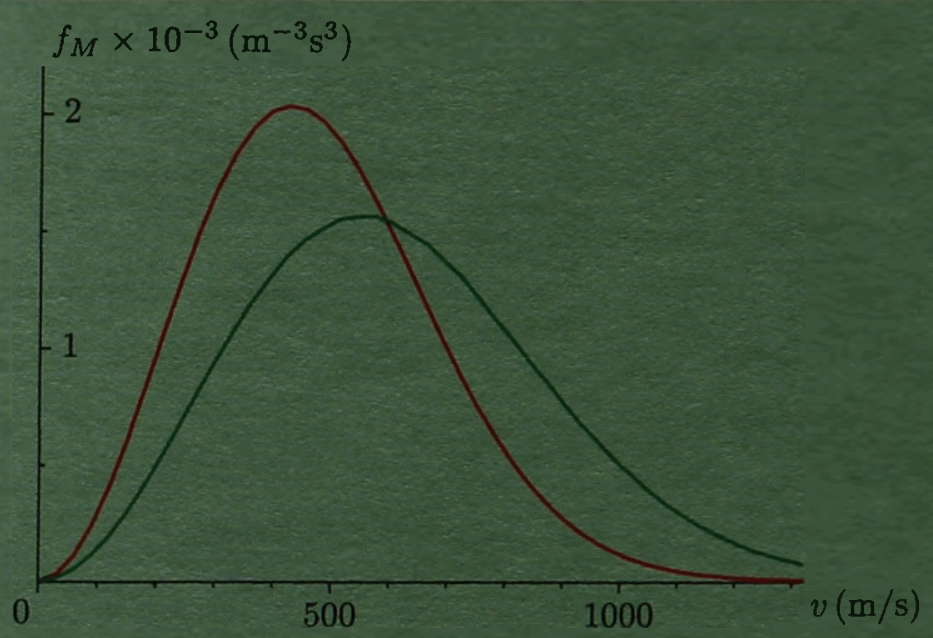
\includegraphics[width=0.4\linewidth]{mai_fig048.png}
   \captionof{figure}{Maxwellovo rozdělení rychlostí molekul dusíku pro teploty \(T_1 = 
                      \SI{300}{\kelvin}\) a \(T_2 = \SI{300}{\kelvin}\).
   \cite[s.~243]{Musilova2009MA1}
   \label{mai:fig048}}
  \par}
  
  Dokážete vyložit, proč jsme zvolili za \(\Delta\Omega\) celý objem slupky? Počítáme totiž 
  pravděpodobnost, že koncový bod vektoru rychlosti molekuly leží, zhruba řečeno, v kterémkoli 
  elementárním kvádříku \(\Delta v_x\Delta v_z\Delta v_z\) obsaženém ve slupce. A ta je součtem 
  pravděpodobností odpovídajících všem kvádříkům vytvářejícím slupku. Jedná se o pravděpodobnosti 
  navzájem neslučitelných jevů (pohybuje-li se molekula v jednom směru, nepohybuje se v jiném). 
  Hustota této pravděpodobnosti se nazývá \textbf{Maxwellovo rozdělení rychlostí}. Na rozdíl od 
  Gaussova rozdělení, popisujícího hustotu pravděpodobnosti pro jednotlivé složky rychlosti, je 
  nesymetrická vlivem faktoru \(v^2\). Obrázek \ref{mai:fig048} ukazuje funkci \(f_M(v)\) pro dvě 
  různé teploty \(T_2 > T_1\). Důležité hodnoty spjaté s tímto rozdělením jsou 
  \textbf{nejpravděpodobnější rychlost} \(v_p\), \textbf{střední rychlost} \(\langle v \rangle\) a 
  \textbf{střední kvadratická rychlost} \(\langle v^2 \rangle\). Platí
  \begin{align*}
    \der{f_M}{v}        &= 0\, \longrightarrow v_P = \sqrt{\dfrac{2kT}{m}},                      \\
    \langle v \rangle   &= \int_{-\infty}^{\infty}vf_M(v)\dd{v} = \sqrt{\dfrac{8kT}{\pi m}},     \\
    \langle v \rangle^2 &= \int_{-\infty}^{\infty}v^2f_M(v)\dd{v} = \dfrac{3kT}{m}.
  \end{align*}
\normalsize
\end{example}
      %---------------------------------------------------------------
  
  \section{Náhoda a zpracování měření}\label{mai:IchapIVsecIV}
    \subsection{Součet a součin náhodných veličin}
      Nyní vyřešíme ještě jeden důležitý problém. Víme již, že veličinu \(Y = f(X)\) lze popsat 
      stejnými pravděpodobnostmi jako veličinu \(X\). V řadě případů je však náhodná veličina \(Y\) 
      funkcí několika náhodných veličin \(X_1, X_2, \ldots, X_s\). Každá z nich má nějaké 
      rozdělení. Jaké potom bude rozdělení veličiny \(Y\)? Rozebereme jen dvě základní situace, z 
      nichž je ovšem možné „poskládat“ řadu případů složitějších. Půjde o situace, kdy náhodná 
      veličina bude součtem nebo součinem dvou náhodných veličin, pro jednoduchost značení 
      například \(U\) a \(V\), tedy \(Y = U + V\), \(Z = U \cdot V\). Předpokládejme nejprve, že 
      veličiny \(U\) a \(V\) jsou zcela nezávislé, tj. hodnoty veličiny \(U\) nejsou nijak 
      ovlivněny hodnotami veličiny \(V\) a naopak. Dejme tomu, že \(U\) a \(V\) mají rozdělení
      \begin{equation*}
        \left\lbrace (u_1, p_1), \ldots, (u_k, p_k) \right\rbrace, \qquad
        \left\lbrace (v_1, q_1), \ldots, (v_\ell, v_\ell) \right\rbrace
      \end{equation*}
      Veličiny \(Y = U + V\), resp. \(Z = U \cdot V\) tedy mohou nabývat hodnot \(\lbrace u_i + 
      v_\alpha\rbrace\), resp. \(\lbrace u_i v_\alpha\rbrace\) s pravděpodobnostmi \(p_iq_\alpha\). 
      Jevy \uv{Veličina \(U\) nabude hodnoty \(u_i\)} a \uv{veličina \(V\) nabude hodnoty 
      \(v_\alpha\)} jsou totiž nezávislé. Rozdělení veličin \(Y\) a \(Z\) je 
      \begin{equation*}
          \begin{rcases}
            \lbrace (u_i +v_\alpha, p_iq_\alpha)\rbrace,\\
            \qquad\text{resp.}\\
            \lbrace(u_iv_\alpha, p_iq_\alpha)\rbrace,
          \end{rcases}
        \begin{array}{c}
          1\leq i\leq k,\\
          1\leq\alpha\leq\ell,
        \end{array}
      \end{equation*}
      Pro jejich střední hodnoty dostáváme
      \begin{align*}
        \langle y \rangle 
          &= \sum_{i=1}^{k}\sum_{\alpha=1}^{\ell}(u_i + v_\alpha)p_iq_\alpha        \\
          &= \sum_{i=1}^{k}u_ip_i\left(\sum_{\alpha=1}^{\ell}q_\alpha\right) + 
             \sum_{\alpha=1}^{\ell}v_\alpha q_\alpha\left(\sum_{i=1}^{k}p_i\right)  \\
          &= \sum_{i=1}^{k}u_ip_i + \sum_{\alpha=1}^{\ell}v_\alpha q_\alpha         \\
        \langle z \rangle 
          &= \sum_{i=1}^{k}\sum_{\alpha=1}^{\ell}(u_i \cdot v_\alpha)p_iq_\alpha    \\
          &= \left(\sum_{i=1}^{k}u_ip_i\right)
             \left(\sum_{\alpha=1}^{\ell}v_\alpha q_\alpha\right) 
           = \langle u \rangle \langle v \rangle.
      \end{align*}
      Střední hodnota součtu, resp. součinu náhodných veličin je tedy součtem, resp. součinem jejich
      středních hodnot. Pro součet náhodných veličin platí tento výsledek i v případě, když nebudou
      nezávislé. V tak jednoduchý závěr jsme snad ani nedoufali! Hned uvidíme, jak jej lze využít.
      
      %--Jak číst výsledky studentské ankety aneb není průměr jako průměr----------
      % !TeX spellcheck = cs_CZ
\wikitextrule
\begin{example}\label{mai:exam071}
  \textbf{Jak číst výsledky studentské ankety aneb není průměr jako průměr}\newline\small
  Každý semestr na Masarykově univerzitě se uzavírá vyhodnocením velmi užitečné studentské ankety v 
  Informačním systému MU. Studenti hodnotí na jedenáctihodnotové stupnici (nula až deset bodů) 
  několik položek pro každý studijní předmět (obtížnost, zajímavost, srozumitelnost výkladu, 
  přístup učitele, rozmanitost literatury) a mohou doplnit i slovní komentáře. Na ty se učitelé 
  těší nejvíce, neboť díky anonymitě pisatelů se tak o sobě mohou dovědět leccos zajímavého. 
  Všimneme si však statistického zpracování ankety. U každého předmětu je pro danou položku 
  vypočtena průměrná bodová hodnota odpovědí a vyznačena na téže jedenáctihodnotové stupnici. Pro 
  porovnání je na stupnici vyznačen i takzvaný „fakultní průměr“. Každý přednášející může vidět svá 
  hodnocení a hodnocení svých kolegů, kteří mu vedou cvičení. Děkan má přístupové právo k celé
  statistice, a tak může porovnávat. Jednoho deštivého večera přestalo děkana bavit vyplňování 
  rektorátních formulářů a začal si výsledky ankety prohlížet. Zajímala jej zejména položka 
  „srozumitelnost výkladu“. Řekl si, že všem učitelům, kteří v této položce budou hodnoceni 
  nadprůměrně, zvýší osobní ohodnocení. Soubor předmětů je veliký, a tak děkan klikal a klikal. 
  Zjišťoval, že u veliké většiny předmětů leží průměrné hodnocení srozumitelnosti nad fakultním 
  průměrem. Jeho pocity byly smíšené. Na jedné straně se radoval, jakými jsou jeho podřízení 
  dobrými pedagogy, na druhé straně trnul, kolik to bude stát. Snad aby se raději vrátil 
  k protivným formulářům. Najednou v něm zahlodalo podezření i naděje, že není všechno v pořádku. 
  Jak je možné, že většina hodnocení leží nad průměrem? Kladné a záporné odchylky by se přece měly 
  kompenzovat. Zavolal proto na koberec proděkana pro informační technologie, aby se jej zeptal, co 
  je to „fakultní průměr“. Proděkan odpověděl takto: Máme soubor \(K\) předmětů \(\lbrace 
  X_\alpha\rbrace\), \(\alpha = 1, \ldots, K\). V předmětu \(X_\alpha\) vyplnilo anketu 
  \(N_\alpha\)  studentů, jednotlivé hodnoty odpovědí pro danou položku (srozumitelnost výkladu) 
  byly označeny \(\lbrace x_{\alpha,j}\rbrace\), \(j = 1, \ldots, N_\alpha\). Celkem přirozeně 
  předpokládáme, že váha odpovědi každého studenta je stejná, nezávisle na předmětu. Tato váha je
  rovna převrácené hodnotě celkového počtu studentů, kteří vyplnili anketu, tj. \(w = N^{-1}\), \(N 
  = N_1 + \ldots + N_k\). Fakultní průměr je proto dán vzorcem
  \begin{equation*}
    \langle x \rangle 
      = \sum_{\alpha=1}^{K}\sum_{j=1}^{N_\alpha}wx_{\alpha,j} 
      = \dfrac{1}{N}\sum_{\alpha=1}^{K}\left(\sum_{j=1}^{N_\alpha}x_{\alpha,j}\right)
      = \dfrac{1}{N}\sum_{\alpha=1}^{K}A_\alpha,
  \end{equation*}
  kde jsme označili \(A_\alpha = \sum_{j=1}^{N_\alpha}x_{\alpha,j}\). Děkan chvíli přemýšlel a 
  pravil: To vypadá docela logicky. Neměli bychom však počítat fakultní průměr tak, že vezmeme 
  průměrné hodnoty pro každý předmět a vypočteme jejich aritmetický průměr? Pak bychom dostali
  \begin{equation*}
    \langle \overline{x} \rangle
      = \dfrac{1}{K}\sum_{\alpha=1}^{K}\langle x_{\alpha}\rangle
      = \dfrac{1}{K}\sum_{\alpha=1}^{K}
        \left(\dfrac{1}{N_\alpha}\sum_{j=1}^{N_\alpha}x_{\alpha,j}\right)
      = \dfrac{1}{K}\sum_{\alpha=1}^{K}\dfrac{A_\alpha}{N_\alpha}.
  \end{equation*}
  Tento závěr se akademickým funkcionářům na první pohled nijak zvlášť nelíbil. Bylo totiž jasné, 
  že náhodné veličiny \(X_1, \ldots, X_k\) mají odlišná rozdělení. No jo, řekli si oba, musíme 
  počítat. My už ale počítat nemusíme, neboť jsme takový problém před chvílí vyřešili obecně. 
  Zjistili jsme totiž, že střední hodnota součtu náhodných veličin je rovna součtu středních 
  hodnot, bez ohledu na konkrétní rozdělení každé z veličin. Definujeme-li tedy náhodnou veličinu 
  \(Y\) jako aritmetický průměr veličin \(X_\alpha\), tj.
  \begin{align*}
    Y &= \dfrac{1}{K}\left(X_1 + \ldots + X_K\right),  \\
    \shortintertext{dostaneme}
    \langle y \rangle &= \dfrac{1}{K}\left(\langle x_1 \rangle +\ldots+\langle x_K \rangle\right).
  \end{align*}
  Tento výsledek se shoduje s hodnotou \(\langle \overline{x} \rangle\), kterou pro výpočet 
  „fakultního průměru“ navrhl děkan. Vypočteme-li součet odchylek hodnot \(\langle x_\beta 
  \rangle\) od \(\langle y \rangle\), dostaneme skutečně nulu:
  \begin{equation*}
    \sum_{\beta =1}^{K}\left(\langle x_\beta \rangle - \langle y \rangle\right)
      = \sum_{\beta =1}^{K}\left(\dfrac{A_\beta}{N_\beta} 
      - \dfrac{1}{K}\sum_{\alpha=1}^{K}\langle x_\alpha \rangle\right)
      = 0.
  \end{equation*}
  Zkusme se ještě zamyslet nad tím , jak použití „špatného“ fakultního průměru zkreslilo výsledky a 
  proč. Vypočtěme si rozdíl \(\Delta = \langle \overline{x} \rangle - \langle x \rangle\):
  \begin{equation*}
    \Delta = \langle \overline{x} \rangle - \langle x \rangle 
      = \dfrac{1}{K}\sum_{\alpha=1}^{K}\langle x_\alpha \rangle
      - \dfrac{1}{N}\sum_{\alpha=1}^{K}A_\alpha
      = \dfrac{1}{K}\sum_{\alpha=1}^{K}\langle x_\alpha \rangle
      - \dfrac{1}{N}\sum_{\alpha=1}^{K}N_\alpha\langle x_\alpha \rangle
      = \dfrac{1}{K}\sum_{\alpha=1}^{K}\langle x_\alpha\rangle\left(1 - K\dfrac{N_\alpha}{N}\right).
  \end{equation*}
  Platí přitom
  \begin{equation*}
    \sum_{\alpha=1}^{K}\left(1 - K\dfrac{N_\alpha}{N}\right) = 0.
  \end{equation*}
  Pokud by byl počet studentů, kteří vyplnili anketu, ve všech předmětech stejný, tj. \(N_\alpha = 
  \dfrac{N}{K}\) , byla by odchylka \(\Delta\) podle očekávání nulová. Stejná situace by nastala, 
  kdyby byly shodné všechny průměrné hodnoty \(\langle x_\alpha \rangle\). Je-li odchylka 
  \(\Delta\) kladná, je „nesprávný“ fakultní průměr \(\langle x \rangle\) nižší než \(\langle 
  \overline{x} \rangle\). Proto hodnocení jednotlivých předmětů vypadají příznivěji, právě tak, jak 
  to zjistil děkan. Odchylku \(\Delta\) posouvají do kladných hodnot předměty, které hodnotilo málo 
  studentů, a předměty, které měly vysoké hodnocení. Dobře je to vidět na příkladu dvou předmětů, 
  tj. pro \(K = 2\), kde vychází
  \begin{equation*}
    \Delta = \langle \overline{x} \rangle - \langle x \rangle 
           = \dfrac{N_2 - N_1}{2(N_2+N_1)}\left(\langle\overline{x}\rangle-\langle x\rangle\right).
  \end{equation*}
  
  Pro \(N_1\ll N_2\) a \(\langle x_1 \rangle  \gg \langle x_2 \rangle \) bude rozdíl \(\Delta\) 
  skoro polovina hodnoty \(\langle x_1 \rangle\)! U volitelných specializovaných předmětů, které si 
  vybírají jen poměrně malé počty studentů, kteří navíc mají o předmět opravdový zájem a hodnotí 
  jej proto většinou vyšším počtem bodů, je splněno obojí (malý počet hodnotících a vysoké bodové
  hodnocení). Je vidět, že při nesprávně zvoleném výpočtu srovnávací hodnoty (fakultního průměru) 
  mohou právě předměty, jejichž statistický význam je spíše okrajový, ovlivnit celkové hodnocení.
\normalsize
\end{example}
      %----------------------------------------------------------------------------
      
      Pro střední hodnotu součtu a součinu nezávislých náhodných veličin jsme získali velmi
      jednoduché výsledky:
      
      \begin{mdframed}[style=highlight]
        \begin{equation}\label{mai:eq070}
          \langle u + v \rangle = \langle u \rangle + \langle v \rangle\quad
          \langle uv \rangle    = \langle u \rangle \langle v \rangle.
        \end{equation}
      \end{mdframed}
      
      Dokážeme také určit rozptyl veličin \(Y = U + V\) a \(Z = U\cdot V\)? Pro rozptyl každé 
      náhodné veličiny platí obecný vztah (\ref{mai:eq061}). Použijeme jej pro naše konkrétní 
      případy:
      \begin{gather*}
        \begin{align*}
          D(U + V) &= \langle (u + v)^2 \rangle - \langle u + v \rangle^2                     \\
                   &= \langle u^2 + 2uv + v^2 \rangle - \left(\langle u \rangle^2 +
                      \langle 2uv \rangle + \langle v^2 \rangle\right)                        \\
                   &= \left(\langle u^2\rangle - \langle u \rangle^2\right)
                    + \left(\langle v^2\rangle - \langle v \rangle^2\right) = D(U) + D(V).
        \end{align*}
      \end{gather*}
      Pro rozptyl náhodné veličiny \(Z = U \cdot V\) dostaneme
      \begin{align*}
        D(Z)  &= \langle z^2\rangle - \langle z \rangle^2 
               = \langle u^2\rangle\langle v^2\rangle - \langle u \rangle^2 \langle v \rangle^2  \\
              &= \left[D(U) + \langle u^2\rangle\right]\left[D(V) + \langle v^2\rangle\right]
               - \langle u \rangle^2 \langle v \rangle^2                                         \\
              &= D(U)D(V) + \langle u \rangle^2D(V) + \langle v \rangle^2D(U).
      \end{align*}
      Pak
      \begin{mdframed}[style=highlight]
        \begin{equation*}
          \dfrac{D(z)}{ \langle z \rangle^2} = \dfrac{D(U)}{ \langle u \rangle^2} \cdot
            \dfrac{D(V)}{ \langle v \rangle^2} + \dfrac{D(U)}{ \langle u \rangle^2} +
            \dfrac{D(v)}{ \langle v \rangle^2}.
        \end{equation*}
      \end{mdframed}
      Při výpočtu jsme využili vztahu (\ref{mai:eq061}) a vztahů (\ref{mai:eq070}) pro střední 
      hodnotu součtu a součinu náhodných veličin. Pokud mají veličiny \(U\) a \(V\) shodný rozptyl 
      \(D(U) = D(V) = D\), pak je \(D(U + V) = 2D\). V případě součtu s veličin \(Y = X_1 + \cdots 
      + X_s\) se shodným rozptylem \(D\) resp. směrodatnou odchylkou \(\sigma\) dostáváme
      \begin{equation*}
        D(Y) = sD  \Rightarrow \sigma(y) = \sqrt{s}\sigma.
      \end{equation*}
      Znovu připomeňme, že všechny vztahy týkající se součtu a součinu náhodných veličin, které
      jsme zatím získali, platí za předpokladu, že výchozí veličiny, které sčítáme nebo násobíme, 
      jsou nezávislé.
      
      Aniž bychom se podrobněji zabývali vlastnostmi rozdělení závislých veličin, definujeme pro
      ně charakteristiky, které tuto závislost popisují. Nechť \(U\) a \(V\) jsou dvě libovolně 
      náhodné veličiny, ne nutně nezávislé. Míru jejich závislosti určují veličiny
      \begin{subequations}\label{mai:eq071}
        \begin{align}
          \sigma_{uv} 
            &= \langle (u - \langle u \rangle) (v - \langle v \rangle) \rangle,  \\
          \varrho_ {uv}
            &=\dfrac{\sigma(u)}{\sqrt{D(U)D(V)}} = \dfrac{\sigma(u)}{\sigma{D(u)\sigma(v)}}
        \end{align}
      \end{subequations}  
      zvané \textbf{kovariance} a \textbf{korelační koeficient} veličin \(U\) a \(V\). Platí 
      \(\varrho(uv) \leq 1\). Pro nezávislé veličiny vychází \(\sigma(uv) = 0\) a \(\varrho(uv) = 
      0\).
      
      %-- Rozptyl při Bernoulliově pokusu-----------------------------
      % !TeX spellcheck = cs_CZ
\begin{mdframed}[style=mdexam]
  \begin{example}\label{mai:exam072}
    \textbf{Rozptyl při Bernoulliově pokusu}\newline
    V příkladu \ref{mai:exam066} jsme se zajímali o střední hodnotu veličiny \(X\) definované jako
    počet zdarů při \(n\) opakováních Bernoulliova pokusu. Řekli jsme si, že střední hodnota této
    veličiny je \(np\) s tím, že důkaz lze provést přímo na základě definičního vztahu pro střední
    hodnotu matematickou indukcí. Výpočet rozptylu z definičního vztahu bychom jistě snadno dokázali
    zahájit, horší by však bylo dovést jej do konce. Stačí se podívat na začátek výpočtu
    \begin{align*}
      D(X) &= \sum_{j=0}^n \left(x_j - \langle x \rangle\right)^2p_j             \\
           &= \sum_{j=0}^n \left(j - np\right)^2\binom{n}{j}p^j(1 - p)^j,
    \end{align*}
    a nepochybujeme o tom, že tuto sumu nedokážeme spočítat snadno. Protože již však umíme zacházet
    se součtem náhodných veličin, můžeme využít účinného triku. Veličinu \(X\) si představíme jako
    součet
    \begin{equation*}
      X = U_1 + U_2 + \cdots + U_n,
    \end{equation*}
    kde každá z veličin \(U_j\) může nabývat dvou hodnot. Jedničky v případě, že při \(j\)-tém
    opakování pokusu nastal zdar, a nuly v případě, že nastal nezdar. Součet všech veličin \(U_j\)
    pro \(j = 1\) až \(j = n\) pak skutečně znamená celkový počet zdarů při \(n\) opakováních
    pokusu. Jestliže si uvědomíme, že pravděpodobnost zdaru při kterémkoli z opakování je \(p\) a
    pravděpodobnost nezdaru \((1 - p)\), ihned vidíme, že rozdělení každé z veličin \(U_j\) má tvar
    \(\lbrace(1, p), (0, 1 - p)\rbrace\). Platí tedy
    \begin{equation*}
      \langle u_j\rangle = 1\cdot p + 0 \cdot (1 - p) = p,
    \end{equation*}
    \begin{align*}
      D = D(U_j) &= \left( 1 - \langle u_j\rangle\right)^2p 
                  + \left( 0 - \langle u_j\rangle\right)^2(1 - p)   \\
                 &= p(1 - p)^2 + p^2(1 - p) = p(1 - p).
    \end{align*}
    Každé dvě veličiny \(U_i\), \(U_j\) jsou nezávislé, neboť jednotlivá opakování pokusu jsou
    nezávislá. Střední hodnota jejich součtu je: tedy \(np\) (a to souhlasí s informací v příkladu
    \ref{mai:exam066}) a pro rozptyl jejich součtu platí
    \begin{equation*}
      D(X) = nD = np(1 - p).
    \end{equation*}
    Celkově tedy dostáváme
    \begin{equation*}
      \langle x \rangle = np, \; \sigma(x) = \sqrt{np(1 - p)}.
    \end{equation*}
  \end{example}
\end{mdframed}
      %---------------------------------------------------------------
      
      %-- Rozptyl aritmetického průměru-------------------------------
      % !TeX spellcheck = cs_CZ
\begin{mdframed}[style=mdexam]
  \begin{example}\label{mai:exam073}
    \textbf{Rozptyl aritmetického průměru}\newline
    Již v úvodu odstavce o náhodných veličinách jsme konstatovali, že opakujeme-li v nezměněných
    podmínkách měření jisté fyzikální veličiny (délka závěsu kyvadla, proud procházející vodičem,
    napětí na vodiči, atd.), budeme díky náhodným vlivům dostávat pokaždé poněkud jiný výsledek.
    Říkáme, že měření je zatíženo náhodnými chybami. Výsledek získaný při každém opakování lze
    interpretovat jako hodnotu náhodné veličiny. Dejme tomu, že jsme provedli uměření fyzikální
    veličiny \(X\) a získali hodnoty \(x_1\) až \(x_n\) . V praktické situaci budou tyto hodnoty
    většinou navzájem různé, nemusí tomu tak však nutně být. Fyzikální veličinu chceme ovšem
    reprezentovat jediným údajem, a tím bude její střední hodnota, tj.
    \textbf{aritmetický průměr}
    \begin{equation*}
      \langle x \rangle = \dfrac{x_1 + x_2 + \cdots + x_n}{n}.
    \end{equation*}
    Rozptyl veličiny \(X\) je dán vztahem
    \begin{align*}
      D &= D(X)                                                             \\
        &= \dfrac{\left(x_1 - \langle x \rangle\right)^2 + 
                  \left(x_2 - \langle x \rangle\right)^2 + \cdots +
                  \left(x_n - \langle x \rangle\right)^2}{n}.
    \end{align*}
    Víme, že směrodatná odchylka \(\sigma( x ) = \sqrt{D(X)}\) určuje, nakolik jsou jednotlivé
    výsledky měření v průměru odchýleny od střední hodnoty, charakterizuje tedy přesnost každého
    opakování měření. Podívejme se na celou úlohu z jiné strany: Představme si, že sledujeme \(n\)
    po dvou nezávislých náhodných veličin \(X_1\) až \(X_n\) se shodnou střední hodnotou \(\langle
    x_j \rangle = \langle x \rangle\) a shodnou směrodatnou odchylkou \(\sigma(x_j) = \sqrt{D},\, 1
    \leq j \leq n\). Aritmetický průměr těchto veličin,
    \begin{equation*}
      \langle \Xi \rangle = \dfrac{X_1 + X_2 + \cdots + X_n}{n}.
    \end{equation*}
    je tedy rovněž náhodnou veličinou. Pro jeho střední hodnotu, rozptyl a směrodatnou odchylku
    platí
    \begin{align*}
      \langle \xi \rangle 
                  &= \dfrac{n\langle x \rangle}{n}, \\
      D(\Xi)      &= \dfrac{1}{n^2}\cdot D(X_1 + \cdots + X_n)=\dfrac{nD^2}{n^2}=\dfrac{D}{n}, \\
      \sigma(\xi) &= \dfrac{\sigma(x)}{\sqrt{n}}.
    \end{align*}
  \end{example}
\end{mdframed}
      %---------------------------------------------------------------
      
      Můžeme tedy říci, že aritmetický průměr všech výsledků měření dané fyzikální veličiny je
      \(\sqrt{n}\)-krát přesnější než jednotlivý výsledek měření. Jakkoli se toto konstatování zdá 
      intuitivně zřejmé, je třeba je používat s opatrností.
      
      Především je třeba mít na mysli, co toto konstatování znamená. Jeho charakter je totiž
      opět jen pravděpodobnostní. Jestliže jsou jednotlivá měření prováděna za stejných podmínek,
      jsou rozdělení veličin \(X_1\) až \(X_n\) funkcemi téhož typu. Tyto veličiny mají také 
      stejnou střední hodnotu \(\langle x \rangle\) a směrodatnou odchylku \(\sigma\). Také 
      pravděpodobnost, že při měření padne hodnota veličiny \(X_j\) do intervalu \((\langle x 
      \rangle - \sigma, \langle x \rangle + \sigma)\), je pro všechna \(j\) prakticky stejná. 
      Označme ji \(P_\sigma\).  Se stejnou pravděpodobností nabude aritmetický průměr \(\Xi\) 
      hodnoty v intervalu určeném svou směrodatnou odchylkou. Ta je však \(\sqrt{n}\)-krát menší. V 
      tomto smyslu jsou hodnoty aritmetického průměru \uv{\(\sqrt{n}\)-krát méně rozptýleny} kolem 
      střední hodnoty \(\langle\xi \rangle\) než hodnoty náhodných veličin \(X_j\) kolem svých 
      středních hodnot \(\langle x \rangle\).
      
      Dalším problémem může být splnění výchozích předpokladů, které vedly ke vztahu pro
      směrodatnou odchylku aritmetického průměru. Ukážeme to na následujícím příkladu.
      
      %-- Jak přesně lze změřit čínského císaře?----------------------
      % !TeX spellcheck = cs_CZ
\wikitextrule
\begin{example}\label{mai:exam075}
  \textbf{Ověření Ohmová zákona}\newline\small

\normalsize
\end{example}
      %---------------------------------------------------------------
      
      %-- Záhada přijímací zkoušky aneb k čemu může posloužit distribuční funkce-----
      % !TeX spellcheck = cs_CZ
\begin{mdframed}[style=mdexam]
  \begin{example}\label{mai:exam075}
    \textbf{Záhada přijímací zkoušky aneb k čemu může posloužit distribuční funkce?}\newline
    Mohlo by se zdát, že distribuční funkce je jen teoretický pojem a že v praktických situacích ji
    těžko využijeme. Podstatné je přece pravděpodobnostní rozdělení náhodné veličiny a distribuční
    funkce je z něj jen jaksi odvozena sčítáním pravděpodobností (u diskrétního rozdělení) nebo
    integrací (u rozdělení spojitého). Přesvědčíme se, že existují velmi realistické případy, kdy
    distribuční funkce přináší věrohodnější informaci o náhodné veličině než samotné rozdělení.
    
    Na Masarykově univerzitě musí každý uchazeč o studium, ať již se hlásí na přírodovědeckou,
    právnickou, lékařskou či jinou fakultu, absolvovat Test studijních předpokladů. Jedná se o
    všeobecný test, zaměřený na zjišťování úrovně všech schopností uchazeče, které jsou potřebné pro
    univerzitní studium, například analytického myšlení, verbálních schopností, numerického myšlení,
    geometrické představivosti, atd. Pro nás však v tu to chvíli není podstatný obsah testu, ale
    způsob zpracování jeho výsledků a vyhodnocení pořadí uchazečů. Test skládá kolem třiceti tisíc
    studentů. Není tedy možné technicky zajistit, aby proběhl v jediné variantě v jednom dni. K
    dispozici je proto osm variant testu, každou variantu řeší tři až čtyři tisíce studentů. Test má
    \num{80} otázek, základním údajem pro zpracování jeho výsledků je počet správných odpovědí
    každého studenta. Pokud bychom označili jako \(i\) počet správných odpovědí (\(i \in\lbrace0, 1,
    2, \ldots, 80\rbrace\)) v kterékoli variantě a \(\mathcal{N}_i\) počet studentů, kteří dosáhli
    právě \(i\) správných odpovědí, dostaneme náhodnou veličinu \(X_i\), kterou bychom mohli nazvat
    „počet správných odpovědí“, pro celou univerzitu. Její rozdělení by mělo tvar
    \begin{equation*}
      \lbrace(i,p_i)\rbrace,\quad\text{kde}\qquad p_i = \dfrac{\mathcal{N}_i}{\mathcal{N}}, \quad
      \mathcal{N} = \sum_{i=0}^{80}\mathcal{N}_i
    \end{equation*}
    A zde je malý „kámen úrazu“. A by bylo možné sestavit opravdu „univerzální pořadí“, musely by
    být všechny varianty testu ekvivalentní z hlediska obtížnosti. To znamená, že kdyby kterýkoli
    student vyplnil za stejných podmínek všechny varianty, dosáhl by v každé z nich stejného počtu
    správných odpovědí s pravděpodobností velmi blízkou jedné. Skutečnost je však principiálně
    taková, že u sebelépe promyšleného a sestaveného testu se jednotlivé varianty budou mírně, v
    rámci statistických, a tedy již neodstranitelných, odchylek lišit. Tato odlišnost se nepozná
    předem, ale až po zpracování výsledků všech variant. Použít pro stanovení pořadí uchazečů
    rozdělení náhodné veličiny \(X\) \emph{= počet správných odpovědí je tedy nespravedlivé}.
    Student, který řešil variantu „statisticky obtížnější“, by v pořadí skončil s horším umístěním,
    než student, který je stejně schopný, avšak měl to štěstí, že na něj připadla varianta
    „statisticky méně obtížná“. Skutečně, kdybychom sestavili grafy rozdělení náhodných veličin
    \(X^{(\alpha)}\) \emph{= počet správných odpovědí v \(\alpha\)-té variantě},
    \begin{equation*}
      \lbrace(i,p_i^{(\alpha)})\rbrace,\quad\text{kde}\; 
      p_i^{(\alpha)} = \dfrac{\mathcal{N}_i^{(\alpha)}}{\mathcal{N}^{(\alpha)}}, \quad
      \mathcal{N}^{(\alpha)} = \sum_{i=0}^{80}\mathcal{N}_i^{(\alpha)}
    \end{equation*}
    zjistili bychom, že se mírně liší. (V předchozím zápisu značí \(\mathcal{N}_i^{(\alpha)}\) počet
    studentů, kteří odpověděli správně na \(i\) otázek \(\alpha\)-té varianty
    \(\mathcal{N}^{(\alpha)}\) je počet všech studentů, kteří tuto variantu řešili.) Střední hodnoty
    i mediány náhodných veličin se i při vynikající shodě obtížnosti všech variant mohou lišit v
    rozmezí jedné až dvou správných odpovědí. A s ohledem na skutečnost, že každou variantu řeší
    obrovský počet studentů, až čtyři tisíce, je zřejmé, že tento rozdíl může poněkud „zamíchat
    “pořadím, zejména v blízkosti mediánu, kde se týká třeba i tří stovek studentů v každé variantě.
    Situaci dokládá obrázek \ref{mai:fig049}. Jak tedy zařídit, abychom dostali spravedlivé pořadí?
    Jediný rozumný způsob, jak minimalizovat vliv statistických odchylek obtížnosti jednotlivých
    variant, je nehodnotit studenty podle absolutního počtu správných odpovědí, ale nějak je
    porovnat mezi sebou. Budeme při tom předpokládat, že rozložení schopností studentů je ve všech
    osmi skupinách, které řeší osm daných variant, stejné. Řeknete si - zase nějaké další
    předpoklady. To je jako z bláta do louže. Předpoklad o stejném rozložení schopností studentů v
    tak velkých skupinách, jako jsou ty naše, je však mnohem realističtější než předpoklad o
    dokonalé shodě obtížnosti variant testu. Budeme se jej proto držet. Každému studentovi
    přisoudíme číslo, které informuje o tom, kolik řešitelů dané varianty bylo horších nebo stejně
    dobrých jako on, tj. mělo nižší nebo stejný počet správných odpovědí. Z matematického hlediska
    to znamená přejít v každé variantě od rozdělení k distribuční funkci. Věnujme se nyní tomuto
    přepočtu podrobněji jak pro diskrétní rozdělení náhodné veličiny \(X^{(\alpha)}\), které
    odpovídá skutečné situaci, tak pro zajímavost i pro rozdělení spojité. V dalším budeme vždy
    zpracovávat výsledky jedné varianty, upustíme proto od vyznačování indexu \(\alpha\).

    {\centering
    \captionsetup{type=figure}
    \luafigure[0.8]{mai_fig049.png}
    \captionof{figure}{Rozdělení pro dvě varianty testu,
    \cite[s.~252]{Musilova2009MA1}
    \label{mai:fig049}}
    \par}
    
    \textbf{Diskrétní rozdělení}
      \begin{itemize}
        \item \emph{Zadání:} Skupina \(N\) studentů řeší jednu variantu testu. Test má \(Q\) otázek.
              Za každou správnou odpověď je přidělen jeden výchozí bod. Získáváme rozdělení
              \begin{gather*}
                \left\lbrace\left(i, \dfrac{N_i}{N} \right)\right\rbrace, \;
                i\in\lbrace0, 1, 2, \ldots, Q\rbrace, \;
                \sum_{i=0}^{Q}N_i = N 
              \end{gather*}
              kde \(i\) je počet výchozích bodů a \(N_i\) počet studentů, kteří získali \(i\) bodů.
              Distribuční funkce tohoto rozdělení
              \begin{gather*}
                F(x) = \dfrac{1}{N}\sum_{i=0}^{j}N_i\;\text{ pro }\;
                j\leq x < j+1, \; x\in\left[0,\infty\right)
              \end{gather*}
              Pro uchazeče, který získal \(j\) bodů, mají význam následující hodnoty:
              \begin{itemize}
                \item \(F(x)    x \in \left[j, j+1\right)\): poměrný počet uchazečů, kteří získali
                      počet výchozích bodů nižší nebo shodný s daným uchazečem,
                \item \(NF(x)   x \in \left[j, j+1\right)\): absolutní počet uchazečů, kteří získali
                      počet výchozích bodů nižší nebo shodný s daným uchazečem,
                \item \(100F(x) x \in \left[j, j+1\right)\): absolutní počet uchazečů, kteří získali
                      počet výchozích bodů nižší nebo shodný s daným uchazečem,
              \end{itemize}
        \item Hodnoty distribuční funkce můžeme získat z následující tabulky:
        
              {\centering
                \resizebox{0.8\textwidth}{!}{%
                \begin{tabular}{c|c}
                          interval \(x\)     &  \(NF(x)\)         \\ \hline
                  \(\left[0,1\right)\)       &  \(N_0\)           \\ 
                  \(\left[1,2\right)\)       &  \(N_0 + N_1\)     \\ 
                  \(\cdots\)                 &  \(\cdots\)        \\
                  \(\left[j,j+1\right)\)     &  \(N_0 + N_1 + \cdots + N_j\) \\ 
                  \(\cdots\)                 &  \(\cdots\) \\
                  \(\left[Q-1,Q\right)\)     &  \(N_0 + N_1 + \cdots + N_{Q-1}\) \\ 
                  \(\left[Q,\infty\right)\)  &  \(N_0 + N_1 + \cdots + N_{Q} = N\) 
                \end{tabular}}
              \par}
        \item Přepočet hodnocení uchazečů tak, aby nová stupnice byla opět v rozsahu mezi nulou a
              \(Q\) a aby nové hodnocení bylo opět celočíselné, je následující:
              \begin{equation*}
                y =QF(x), \quad 0\leq F(x) \leq 1, \Rightarrow y \in[0,Q].
              \end{equation*}
              Uchazeči se ziskem \(i\) výchozích bodů náleží hodnota \(y = QF(x)\) právě když i\(
              \in \left[i, i + 1\right)\), tj. \(y_i = Q F(i)\). Tato hodnota není obecně
              celočíselná. Zaokrouhlení se provede ve prospěch uchazeče, tedy vždy nahoru. Výsledný
              převodní vzorec je
              \begin{equation*}
                \begin{multlined}
                  \text{výchozí body } i \longrightarrow\text{ nové body }  \\ 
                  \shoveleft[1cm]Y_i: Y_i = [y_i] + 1 = [QF(i)] + 1,
                \end{multlined}
              \end{equation*} 
              kde \([a]\) značí celočíselnou část čísla \(a\), tedy například \([\num{23.05}] =
              [\num{23.48}] = [23,89] = 23\)
        \item Zaveďme novou náhodnou veličinu \(Z\) s rozdělením \(\left\lbrace(z_\alpha,
              M_\alpha)\right\rbrace\): Označme \(z_1, z_2, \ldots, z_\alpha, ...,\) \(z_S\)
              navzájem různé hodnoty ze souboru \(\lbrace Y_i\rbrace, i = 0, 1, 2, \ldots, Q\)
              řazené vzestupně. Její rozdělení udává kterákoli z následujících tabulek:

              {\centering
                \resizebox{0.9\textwidth}{!}{%
                \begin{tabular}{c|c}
                          hodnota                       &  četnost         \\
                          \hline
                  \(z_1 = Y_0 = Y_1 = \cdots Y_{i_1}\)  & \(M_1 = N_0 + N_1 + \cdots + N_{i_1}\)  \\ 
                  \(Z_2 = Y_{i_1+1} = \cdots Y_{i_2}\)  & \(M_2 = N_{i_1+1} + \cdots + N_{i_2}\)  \\ 
                  \(\cdots\)                            & \(\cdots\)                              \\
                  \(Z_S = Y_{i_{S-1}+1}=\cdots Y_{i_S}\)& \(M_S = N_{i_{S_1}+1}+\cdots+N_{i_S}\)   
                \end{tabular}}
              \par}

              {\centering
                \resizebox{0.9\textwidth}{!}{%
                \begin{tabular}{c|c}
                          hodnota                        &  četnost         \\
                          \hline
                  \(z_1 = Y_0 = Y_1 = \cdots Y_{i_1}\)   &  \(M_1 = NF(i_1)\)              \\
                  
                  \(Z_2 = Y_{i_1+1} = \cdots Y_{i_2}\)   &  \(M_2 = N[F(i_2) - F(i_1)]\)  \\ 
                  \(\cdots\)                             &  \(\cdots\)                     \\
                  \(Z_S = Y_{i_{S-1}+1}=\cdots Y_{i_S}\) & \(M_S = N[F(i_S) - F(i_{S-1})]\)   
                \end{tabular}}
              \par}
              kde \(i_1 < i_2 < \ldots < i_{S-1} < i_S, i_S = Q\) (Vzhledem k zaokrouhlování nahoru
              není žádná bodová hodnota \(Y_i\) nulová.) I když skutečné rozdělení při zpracování
              výsledků testů je diskrétní, ukažme si, jak by vypadal analogický postup u rozdělení
              spojitého, kde je početní zpracování názornější.
      \end{itemize}
    
    \textbf{Spojité rozdělení}
      \begin{itemize}
        \item \emph{Zadání:} Je dáno rozdělení četností \(n(x) \leq 0,\, x \in [0, Q]\).
        \item Normovací podmínka a distribuční funkce jsou
              \begin{equation*}
                \int_{0}^{Q}n(x)\dd{x} = N, \quad 
                F(x) = \dfrac{1}{n}\int_{0}^{x}n(\xi)\dd{\xi},                
              \end{equation*}
              kde \(0 \leq F(x) \leq 1.\)
        \item Označme \(z = QF(x)\), tedy \(z \in [0, Q]\), novou náhodnou veličinu. (Uvědomme si,
              že \(z\) je rostoucí funkcí proměnné \(x\)). Označme její rozdělení \(\nu(z)\). Její
              distribuční funkce je
              \begin{align*}
                \Phi(z) &= \int_{0}^{z}\nu(\zeta)\dd{\zeta} 
                         = \int_{0}^{x(z)}\dfrac{n(\xi)}{N}\dd{\xi}          \\
                        &= F\left(F^{-1}(z/Q)\right) 
                        = \dfrac{z}{Q}, \quad
                \nu(z) = \dfrac{1}{Q}.
              \end{align*}
        \item Rozdělení je konstantní s mediánem i střední hodnotou \(Q/2\). Takové rozdělení se
              nazývá rovnoměrné.
      \end{itemize}
  \end{example}
\end{mdframed}
      %------------------------------------------------------------------------------
      
    \subsection{Který výsledek je ten pravý?}
      První věc, kterou budete dělat ve fyzikálním praktiku, bude zjišťování průměrné hustoty 
      materiálu, z něhož je vyroben kovový váleček. Budete váleček vážit, abyste určili jeho 
      hmotnost,a měřit jeho výšku a průměr, abyste mohli vypočítat jeho objem. Hustotu stanovíte 
      jako podíl hmotnosti a objemu. Jedná se stále o jeden a týž váleček, jehož průměrná hustota 
      má za daných podmínek (stálá teplota, váleček se nedeformuje, apod.) stále stejnou „správnou“ 
      hodnotu, kterou však neznáme. (Nezná ji ani učitel v praktiku, i když se tak tváří.) Změří-li 
      hustotu válečku všichni studenti ve skupině, každý jen jednou, získá se řada různých hodnot. 
      Která z nich je ta správná? Není vyloučeno, a je to dokonce velmi pravděpodobné, že žádná. A 
      mohli bychom pomocí nich správnou hodnotu určit nebo se k ní alespoň přiblížit? Možné by to 
      bylo, pokud bychom zaručili, že všechny výsledky získané jednotlivými studenty jsou „stejně 
      hodnotné“. Znamenalo by to, že bychom museli vyloučit hrubé a systematické chyby, které by 
      vznikly třeba tak, že by někteří studenti vážili na vadných vahách, někteří by měli špatné 
      měřítko, popřípadě by odečítali údaj „zboku“, takže by byl zkreslený, nebo by se dokonce 
      zmýlili při odečítání údaje. Museli bychom také zaručit, že náhodné vlivy, které ovlivňují 
      měření, zatěžují je náhodnými chybami a v principu je nelze odstranit, byly při všech 
      měřeních stejné. U různých studentů si tím však nemůžeme být jisti (vzpomeňte si na měření 
      čínského císaře), proto budeme raději postupovat tak, že jeden pečlivý student provede větší 
      počet měření třeba výšky válečku, která je pro určení hustoty potřebná. Dejme tomu, že bude 
      měřit milimetrovým měřítkem a bude odhadovat s přesností na půl milimetru. Jeho údaje tedy 
      mohou mít tvar \SI{33.0}{\mm}, \SI{34.5}{\mm}, atd. Získá takto za stejných podmínek třeba 
      dvacet nebo i padesát hodnot, ale co teď s nimi? Jak určit hodnotu, která se bude nejvíce 
      blížit správné hodnotě výšky válečku? (Dalo by se jistě diskutovat i o tom, co je to správná 
      hodnota. Pro tuto chvíli však předpokládejme, že taková hodnota skutečně existuje, neboť 
      váleček je opravdu válcem, je vysoustružen pečlivě, přesněji, než jsme schopni jej měřit, při 
      měření se nemění teplota, váleček není dáván do lisu a deformován, ani upravován tak, že by 
      se měnila jeho hmotnost.) Předpokládejme, že správná hodnota výšky válečku je \(x\) a že 
      student naměřil hodnoty \(\lbrace x_1, X_2, \ldots, x_n\rbrace\), mezi nimiž mohou být 
      pochopitelně i některé hodnoty stejné. Odchylky jeho měření od správné hodnoty jsou
      \begin{equation*}
        \lbrace \varepsilon_1, \varepsilon_2, \ldots, \varepsilon_n\rbrace, \qquad
        \varepsilon_i = x_i - x, \qquad i = 1, 2, \ldots, n.
      \end{equation*}
      I kdybychom správnou hodnotu \(x\) znali, nedokázali bychom předpovědět, nakolik se od ní při
      jednotlivém měření odchýlíme. Můžeme, se však zajímat o to, jaká je pravděpodobnost, že
      hodnota, o kterou bude měření od správné hodnoty odkloněno, bude ležet v určitém intervalu.
      Odchylky \(\varepsilon_i\) lze totiž interpretovat jako hodnoty náhodné veličiny. Abychom 
      mohli požadované pravděpodobnosti určit, potřebujeme znát rozdělení této veličiny. Označme ji 
      \(\varepsilon\) a odpovídající hustotu pravděpodobnosti \(\mathcal{w}(\varepsilon)\). Toto 
      rozdělení je za určitých podmínek \textbf{rozdělením normálním}, splňuje tedy vztah 
      (\ref{mai:eq069}). Zkusme se o tom přesvědčit. Zvolme podmínky měření tak, aby byly ve hře 
      jen náhodné chyby způsobené \(m\) nezávislými vlivy. Každý z nich hodnotu měření
      odchýlí od \(x\) o stejně velkou hodnotu \(\alpha\), kladnou nebo zápornou, s 
      pravděpodobností \num{0.5}. Schéma této úvahy je na obrázku \ref{mai:fig050}. Výsledná 
      odchylka naměřené hodnoty \(x_i\) od hodnoty správné s jistotou leží v intervalu \((-m\alpha, 
      m\alpha)\) a může nabývat pouze hodnot celých násobků \(\alpha\). Při uplatnění jednotlivého 
      „chybového“ vlivu vzniká, jak jsme již řekli, kladná nebo záporná odchylka o velikosti 
      \(\alpha\). Vznik odchylky \(+\alpha\) nazveme zdarem, vznik odchylky \(-\alpha\) nezdarem.
      
      \luagraphic[1]{mai_fig050.png}{Vznik kladných a záporných odchylek při měření s \(m\) vlivy. 
      \cite[s.~255]{Musilova2009MA1}}{mai:fig050}
     
      Mohlo by tomu být i naopak, slova „zdar“ a „nezdar“ zde nemají svůj obvyklý význam, jde
      pouze o to, že díky nim můžeme hned uvidět souvislost s Bernoulliovým pokusem a tedy
      i s Bernoulliovým rozdělením. Při \(j\) kladných a \(m - j\) záporných odchylkách je měření od
      správné hodnoty odkloněno o
      \begin{equation*}
        j\alpha + (m - j)(-\alpha) = (2j - m)\alpha
      \end{equation*}
      s pravděpodobností
      \begin{equation*}
        p_j = \binom{m}{j}p^j(1 - p)^{m - j} = 2^{-m}.
      \end{equation*}
      Střední hodnota náhodné veličiny \(\varepsilon\) je nulová. Skutečně, v příkladu 
      \ref{mai:exam066} jsme zjistili, že střední hodnota veličiny \(Y\) nabývající hodnot \(y_j = 
      j\) s Bernoulliovým rozdělením je \(\langle y \rangle = mp\), střední hodnota veličiny \((2j 
      - m)\) a pak musí být \((2mp - m)\alpha\). Pro \(p = \num{0.5}\) je tato hodnota nulová.
      Pro velká \(m\) lze Bernoulliovo rozdělení nahradit rozdělením normálním (obr. 3.8), a proto 
      má náhodná veličina \(\varepsilon\) hustotu pravděpodobnosti tvaru (\ref{mai:eq069}), tj.
      \begin{equation*}
        \mathcal{w}(\varepsilon) = 
        \dfrac{1}{\sigma\sqrt{2\pi}}\exp\left(\dfrac{-\varepsilon^2}{2\sigma^2}\right).   
      \end{equation*}

      \luagraphic[0.8]{mai_fig051.png}{Normální rozdělení jako limitní případ Bernoulliova 
      \cite[s.~256]{Musilova2009MA1}}{mai:fig051}
    
      Vraťme se nyní k otázce zpracování naměřených hodnot \(\lbrace x_1, \ldots, x_n\rbrace\) 
      výšky válečku. Jejich odchylky od správné hodnoty jsou \(x_1 - x\) až \(x_n - x\). Na místě 
      neznámé správné hodnoty \(x\) si nyní představme nějakou proměnnou, označme ji 
      \(\varepsilon\). Budeme se snažit určit její hodnotu \(\varepsilon_0\) tak, aby 
      pravděpodobnost, že odchylky jednotlivých měřených hodnot od \(\varepsilon_0\) padnou 
      současně do intervalů
      \begin{equation*}
        \begin{multlined}
          \left(\varepsilon_1 - \dfrac{\dd{\varepsilon_1}}{2}, 
                \varepsilon_1 + \dfrac{\dd{\varepsilon_1}}{2}
          \right),
          \left(\varepsilon_2 - \dfrac{\dd{\varepsilon_2}}{2}, 
                \varepsilon_2 + \dfrac{\dd{\varepsilon_2}}{2}
          \right), \cdots, \\
          \shoveleft[0.5cm]\left(\varepsilon_n - \dfrac{\dd{\varepsilon_n}}{2}, 
                                \varepsilon_n + \dfrac{\dd{\varepsilon_n}}{2}
                          \right),          
        \end{multlined}
      \end{equation*}
      byla maximální. Pro tuto pravděpodobnost v závislosti na \(\xi\) platí
      \begin{gather}
        \begin{aligned}
          \dd{W} &= \dd{\mathcal{w}(\varepsilon_1)}\cdots\dd{\mathcal{w}(\varepsilon_n)} \nonumber\\
                 &= \dfrac{1}{\sigma\sqrt{2\pi}}
                    \exp\left(-\dfrac{(x_1 - \xi)^2 + \cdots + (x_n - \xi)^2}{2\sigma^2}
                        \right)\dd{\varepsilon_1}\cdots\dd{\varepsilon_n}.      \label{mai:eq072}
        \end{aligned}
      \end{gather}
      (Víte proč je ve vztahu (\ref{mai:eq072}) součin pravděpodobností?) Tato pravděpodobnost bude 
      maximální, bude-li hodnota exponentu minimální. Z podmínky
      \begin{equation*}
        (x_1 - \xi)^2 + \cdots + (x_n - \xi)^2 = \text{min}
      \end{equation*}
      dostáváme derivací podle \(\xi\) požadavek
      \begin{equation*}
        2(x_1 - \xi) + \cdots + 2(x_n - \xi) = 0 \Rightarrow \xi_0 = 
        \dfrac{1}{n}\sum_{i=1}^{n}x_j = \langle x \rangle.
      \end{equation*}
      Vidíme, že veličina, která charakterizuje míru odchýlení naměřených hodnot od \(\xi\), je 
      minimální, zvolíme-li za \(\xi\) aritmetický průměr naměřených hodnot. Pozor, zjištěný 
      výsledek znamená právě jen konstatovanou skutečnost: Při dosazení aritmetického průměru za 
      proměnnou \(\xi\) bude pravděpodobnost, že odchylky jednotlivých měření od \(\xi\) budou 
      ležet v uvažovaných intervalech, maximální. Neznamená to, že správnou hodnotou veličiny \(X\) 
      je aritmetický průměr měření \(x_1, X_2, \ldots, x_n\). Správnou hodnotu ze souboru měření 
      prostě nezjistíme, avšak aritmetický průměr je jí blízký s vysokou pravděpodobností. Jaká je 
      tato „blízkost“ a její pravděpodobnost konkrétně? Hned uvidíme. Správnou hodnotu výšky 
      válečku \(x\) sice neznáme, ale víme, že náhodná veličina \(\varepsilon\), jejíž hodnoty jsou 
      odchylkami výsledků měření od této (neznámé) správné hodnoty, se řídí normálním rozdělením s 
      nulovou střední hodnotou. Potřebujeme stanovit další důležitý parametr tohoto rozdělení, 
      směrodatnou odchylku \(\sigma\). Tu lze vyjádřit velmi jednoduše. Je totiž střední hodnotou 
      náhodné veličiny \(\varepsilon^2\), tedy aritmetickým průměrem čtverců odchylek 
      \(\varepsilon_i\): 
      \begin{equation*}
        \sigma^2 = D(\varepsilon) = \dfrac{1}{n}\sum_{i=1}^{n}\varepsilon_i^2.
      \end{equation*}
      Ať je však tento vzorec jakkoli jednoduchý, k čemu může sloužit, nedokážeme-li jej vyčíslit?
      Když přece neznáme správnou hodnotu \(x\), nemáme k dispozici ani hodnoty \(\varepsilon_i\). 
      Ani tato kaše však není tak horká, jak se zdá: Odchylku výsledku \(i\)-tého měření od 
      aritmetického průměru označme \(\delta_i = x_i - \langle x \rangle\), přičemž jsme již dříve 
      označili jako \(\varepsilon_i= x_i - x\) odchylku výsledku \(i\)-tého měření pd správné 
      hodnoty. Platí
      \begin{equation*}
        \sum_{i=1}^{n}\varepsilon_i = \sum_{i=1}^{n}(x_i - x) \Rightarrow 
        \sum_{i=1}^{n}x_i = \sum_{i=1}^{n}\varepsilon_i + nx, 
      \end{equation*}
      odkud 
      \begin{equation*}
        \langle x \rangle = x + \dfrac{1}{n}\sum_{i=1}^{n}\varepsilon_i.
      \end{equation*}
      Pak dostaneme
      \begin{equation*}
        \delta_i = (x_i - x) - \dfrac{1}{n}\sum_{i=1}^{n}\varepsilon_i 
                 = \varepsilon_i - \dfrac{1}{n}\sum_{j=1}^{n}\varepsilon_j.
      \end{equation*}
      Součet čtverců odchylek \(\delta_i\) je
      \begin{align*}
        \sum_{i=1}^{n}\delta_i^2 
          &= \sum_{i=1}^{n}\left(\varepsilon_i - 
             \dfrac{1}{n}\sum_{j=1}^{n}\varepsilon_j\right)^2 \\
          &= \sum_{i=1}^{n}\varepsilon_i^2 - 
             \dfrac{2}{n}\sum_{i=1}^{n}\sum_{j=1}^{n}\varepsilon_i\varepsilon_j + 
             \dfrac{1}{n^2}\sum_{i=1}^{n}\left(\sum_{j=1}^{n}\varepsilon_j\right)^2     \\
          &= \sum_{i=1}^{n}\varepsilon_i^2 - 
             \dfrac{1}{n}\left(\sum_{j=1}^{n}\varepsilon_j\right)^2                     
             \doteq \left(1 - \dfrac{1}{n}\right)\sum_{i=1}^{n}\varepsilon_i^2.
      \end{align*}
      Při poslední úpravě jsme pro získání výsledného přibližného vyjádření součtu čtverců odchylek
      \(\delta_i\) použili následující úvahy:
      \begin{equation*}
        \left(\sum_{j=1}^{n}\varepsilon_j\right)^2 = \sum_{i=1}^{n}\varepsilon_i^2 + 
        2\sum_{i=1}^{n}\sum_{j>1}\varepsilon_i\varepsilon_j \doteq \sum_{i=1}^{n}\varepsilon_i^2,
      \end{equation*}
      neboť při rovnocenném zastoupení kladných a záporných odchylek je druhý sčítanec, obsahující
      součiny \(\varepsilon_i\varepsilon_j\), zanedbatelný proti prvnímu. Nakonec tedy dostáváme
      \begin{equation*}
        \sum_{i=1}^{n}\delta_i^2 \doteq \dfrac{n-1}{n}\sum_{i=1}^{n}\varepsilon_i^2 = (n-1)\sigma^2.
      \end{equation*}
      Protože odchylky \(\delta_i\) již z daného souboru měření určit můžeme (jsou to odchylky 
      jednotlivých měření od jejich aritmetického průměru), získali jsme alespoň přibližný vztah 
      pro směrodatnou odchylku rozdělení veličiny \(\varepsilon\), 
      \begin{equation}\label{mai:eq074}
        \sigma = \left(\dfrac{1}{n-1}\sum_{i=1}^{n}\delta_i^2\right)^{\dfrac{1}{2}}.
      \end{equation}
      Jaký význam má tato hodnota pro náš soubor měření? Vymezuje interval
      \begin{equation*}
        (x - \sigma, x + \sigma),
      \end{equation*}
      symetrický kolem (stále neznámé) správné hodnoty výšky válečku \(x\), do kterého padne 
      výsledek měření této výšky s pravděpodobností \SI{68.3}{\percent} (příklad 
      \ref{mai:exam069}). Neznámá správná hodnota je tedy naopak s toutéž pravděpodobností vzdálena 
      od výsledku jednotlivého měření o méně než \(\sigma\). A to už je docela slušná informace o 
      tom, kde správná hodnota může ležet. Polohu \(x\) však můžeme „omezit“ ještě lépe. Směrodatná 
      odchylka \(\overline{\sigma}\) rozdělení, které přísluší aritmetickému průměru, je
      totiž ještě \(\sqrt{n}\)-krát menší než \(\sigma\), tj. \(\overline{\sigma}= 
      \sigma/\sqrt{n}\). Správná hodnota \(x\) (navždy neznámá) je tedy od aritmetického průměru 
      výsledků měření \(\langle x \rangle\) vzdálena s pravděpodobností \SI{68.3}{\percent} o méně 
      než \(\overline{\sigma}\). Použijeme-li krajní chybu \(\overline{\kappa} = 
      3\overline{\sigma}\) (příklad \ref{mai:exam069}), můžeme říci, že správná hodnota \(x\) je od
      aritmetického průměru souboru měření \(\langle x \rangle\) vzdálena o méně než 
      \(\overline{\kappa}\) s pravděpodobností \SI{99.7}{\percent}. Více se o správné hodnotě výšky 
      válečku říci nedá. Ale i tak jsme ji lokalizovali docela úspěšně. Následující příklad 
      ukazuje vyhodnocení konkrétního souboru měření.

      %-- Měříme výšku válečku----------------------------------------
      % !TeX spellcheck = cs_CZ
\begin{mdframed}[style=mdexam]
  \begin{example}\label{mai:exam077}
    \textbf{Měříme výšku válečku}\newline
    Student měřil za stejných podmínek výšku válečku dvacetkrát. Při měření byly vyloučeny
    systematické chyby. Měřil tentokrát přesněji - posuvným měřítkem neboli „šuplérou“. Mohl tedy
    odhadovat desetiny milimetru. Získal tyto hodnoty \(x_1\) až \(X_{20}\) v milimetrech (levá část
    tabulky):
    
    {\centering
      \resizebox{\textwidth}{!}{%
      \begin{tabular}{c|ccccc|ccccc}
        \hline
        měření & \multicolumn{5}{l}{\(x_i\) [mm]} & \multicolumn{5}{l}{\(\delta_i\) [mm]} \\ \hline
        1.  až 5.  & \num{35.5} & \num{35.4} & \num{34.9} & \num{35.7} &
                  \num{36.0} & \num{0.2}  & \num{0.1}  & \num{-0.4} & \num{0.4}
                  & \num{0.7}     \\
        6.  až 10. & \num{35.8} & \num{35.2} & \num{35.2} & \num{34.8} &
                  \num{35.0} & \num{0.5}  & \num{-0.1} & \num{-0.1} & \num{-0.5}
                  & \num{-0.3}    \\
        11. až 15. & \num{35.5} & \num{34.8} & \num{35.1} & \num{35.3} &
                  \num{34.9} & \num{0.2}  & \num{-0.5} & \num{-0.2} & \num{0.0}
                  & \num{-0.4}    \\
        16. až 20. & \num{35.8} & \num{35.4} & \num{35.8} & \num{34.8} &
                  \num{35.1} & \num{0.5}  & \num{0.1}  & \num{0.5}  & \num{-0.5}
                  & \num{-0.2}    \\ \hline
      \end{tabular}}
    \par}
    \vspace{\baselineskip}
    Aritmetický průměr těchto hodnot je \(\langle x\rangle = \qty{35.30}{\mm}\). Uvádíme jej zatím s
    přesností o jedno desetinné místo „lepší“ , než jsou jednotlivá měření, neboť ještě nevíme, jak
    dopadnou výpočty chyb. V pravé části tabulky jsou hodnoty \(\delta_i\), tj. odchylky
    jednotlivých měření od aritmetického průměru. Snadno se přesvědčíme, že jejich součet je nulový,
    přesně, jak má být. Směrodatná odchylka vychází \(\sigma \doteq \qty{0.381}{\mm}\) pro jednotlivé
    měření, pro aritmetický průměr pak \(\overline{\sigma} \doteq \qty{0.085}{\mm}\). Na rozdíl od
    hodnot měření se výsledné chyby měření zaokrouhlují vždy nahoru, a to na jedno platné místo.
    (Zaokrouhlujeme nahoru proto, abychom zajistili, že správná hodnota veličiny leží v intervalu
    určeném chybou nejméně s pravděpodobností, která této chybě odpovídá. Po zaokrouhlení tedy máme
    \(\sigma \doteq \qty{0.4}{\mm}\) a \(\overline{\sigma} = \qty{0.09}{\mm}\). Změřenou výšku válečku
    pak zapisujeme takto:
    \begin{equation*}
      \text{výška válečku } = (\langle x \rangle\pm \overline{\sigma}) = \qty{35.30 \pm 0.09}{\mm}.
    \end{equation*}
    Z předchozích úvah víme, jak je nutno takový zápis interpretovat:
    \begin{itemize}
      \item Správná hodnota výšky válečku leží v intervalu \SIrange[range-units =
            brackets]{35.21}{35.39}{\mm} a pravděpodobností nejméně \qty{68.3}{\percent}.
    \end{itemize}
    Při použití krajní chyby, tj. \(\overline{\kappa} \doteq \qty{0.27}{\mm} \doteq \qty{0.3}{\mm}\),
    konstatujeme, že
    \begin{itemize}
      \item Správná hodnota výšky válečku leží v intervalu \SIrange[range-units =
            brackets]{35.0}{35.6}{\mm} s pravděpodobnosti nejméně \qty{99.7}{\percent}.
    \end{itemize}
    Pozn.: Při zcela korektním přístupu ke zpracování laboratorních měření je třeba uvážit, že
    intervaly se stejným pravděpodobnostním obsahem \qty{68.3}{\percent}, resp. \qty{99.7}{\percent}
    jsou ve skutečnosti širší. Správně by totiž měly být stanoveny na základě nekonečného počtu
    měření
  \end{example}
\end{mdframed}
      %---------------------------------------------------------------
      Na závěr odstavce si všimneme ještě jedné důležité otázky. Formulujeme ji pro případ určení
      hustoty válečku. Změřili jsme výšku válečku \(x\) a jeho poloměr \(r\), vážením jsme určili 
      také jeho hmotnost \(m\). Získali jsme tak intervaly
      \begin{align*}
          \left(\langle x \rangle - \overline{\sigma}(x), 
                \langle x \rangle + \overline{\sigma}(x)\right)&,  \\ 
          \left(\langle r \rangle - \overline{\sigma}(r), 
                \langle r \rangle + \overline{\sigma}(r)\right)&,   \\ 
          \left(\langle m \rangle - \overline{\sigma}(m), 
                \langle m \rangle + \overline{\sigma}(m)\right)&. 
      \end{align*}
      
      Směrodatná odchylka v případě každé z veličin \(x\), \(r\) a \(m\) určuje velikost intervalu 
      se středem daným aritmetickým průměrem všech měření této veličiny, v němž leží správná 
      hodnota s pravděpodobností \SI{68.3}{\percent}. Průměrná hustota válečku je dána vztahem
      \begin{equation*}
        \varrho = \dfrac{m}{V} = \dfrac{m}{\pi r^2x},
      \end{equation*}
      je tedy funkcí tří proměnných \(x\), \(r\), \(m\). Jak stanovíme interval, v němž leží 
      správná hodnota hustoty s pravděpodobností rovněž \SI{68.3}{\percent}? Hustotu totiž neměříme 
      přímo, ale vypočítáváme z přímo měřených veličin. Abychom mohli na tuto otázku odpovědět 
      matematicky korektně, potřebujeme základní znalosti o funkcích více proměnných. Závěr tohoto 
      odstavce lze tedy do důsledku pochopit po přečtení kapitoly o funkcích více proměnných. Proto 
      jej v tuto chvíli klidně přeskočte.
      
      Předpokládejme, že veličina \(z\) je pro jednoduchost pouze funkcí dvou nezávislých náhodných
      veličin \(x\) a \(y\), \(z = f(x,y)\). Jsou-li chyby \(\varepsilon_i(x)\), resp. 
      \(\varepsilon_i(y)\), kterých jsme se dopustili při \(i\)-tém měření veličiny \(x\), resp. 
      \(y\) velmi malé, můžeme pro vyjádření malé změny veličiny \(z\) způsobené chybami veličin 
      \(x\) a \(y\) použít úplného diferenciálu
      \begin{equation*}
        \dd{z} = \dd{f(x,y)} = \left(\pder{f(x,y)}{x}\right)\dd{x} + 
                               \left(\pder{f(x,y)}{y}\right)\dd{y}
      \end{equation*}
      Pro chybu veličiny \(z\) pak platí
      \begin{equation*}
        \varepsilon_i(z) = \left(\pder{f}{x}\right)\varepsilon_i(x) + 
                           \left(\pder{f}{y}\right)\varepsilon_i(y) \Rightarrow
      \end{equation*}
      \begin{gather*}
        \begin{align*}
          \Rightarrow \sum_{i=1}^{n}\varepsilon_i^2(z) 
          &=  \sum_{i=1}^{n}\left(\pder{f}{x}\right)^2\varepsilon_i^2(x) 
           +  \sum_{i=1}^{n}\left(\pder{f}{y}\right)^2\varepsilon_i^2(y)    \\
          &+ 2\sum_{i=1}^{n}\left(\pder{f}{x}\right)^2\left(\pder{f}{y}\right)^2\varepsilon_i(x)
            \varepsilon_i(y).
        \end{align*}
      \end{gather*}
      Vzhledem k rovnocennému zastoupení kladných a záporných odchylek je součet obsahující
      součiny \(\varepsilon_i(x)\varepsilon_i(y)\) zanedbatelný proti zbytku výrazu. Pak
      \begin{align*}
        \sum_{i=1}^{n}\varepsilon_i^2(z) 
          &\doteq \left(\pder{f}{x}\right)^2 \sum_{i=1}^{n}\varepsilon_i^2(x) + 
                  \left(\pder{f}{y}\right)^2\sum_{i=1}^{n}\varepsilon_i^2(y)                 \\ 
          &= \left(\pder{f}{x}\right)^2 n\sigma^2(x) + \left(\pder{f}{y}\right)^2n\sigma^2(y).
      \end{align*}
      Odtud, vzhledem k platnosti vztahu
      \begin{equation*}
        \sum_{i=1}^{n}\varepsilon_i^2 = n\sigma^2(z),
      \end{equation*}
      dostáváme
      \begin{equation}\label{mai:eq075}
        \sigma^2(z) = \left(\pder{f}{x}\right)^2\sigma^2(x)
                    + \left(\pder{f}{y}\right)^2\sigma^2(y).
      \end{equation}
      Parciální derivace funkce \(f(x, y)\) podle \(x\), resp. \(y\) je třeba vyčíslit dosazením 
      \(x = \langle x\rangle\) a \(y = \langle y \rangle\). Zobecnění tohoto vzorce na případ, kdy 
      hledaná veličina je funkcí více proměnných, je jednoduché.
      
    \subsection{Lineární závislost a metoda nejmenších čtverců}
      Tento poslední odstavec se zabývá zpracováním měření veličin, které jsou vázány lineárním
      vztahem (už zase ta linearita). Situaci si opět snadno představíme na jednoduchém příkladu
      Víme, že pro elektrické vodiče platí za jistých okolností \emph{Ohmův zákon}. Podle něj je 
      proud \(I\) protékající vodičem, třeba drátem, přímo úměrný napětí \(U\) mezi konci vodiče. 
      Konstanta úměrnosti ve vztahu
      \begin{equation*}
        U = R\cdot I
      \end{equation*}
      představuje \emph{elektrický odpor vodiče} \(R\). Změříme-li napětí a proud, můžeme určit 
      odpor vodiče, pokud Ohmův zákon opravdu platí. Mohli bychom tedy postupovat například tak, že 
      bychom při několika různých hodnotách napětí \(\lbrace U_1, U_2, \ldots, U_n \rbrace\) 
      (napětí bychom mohli například postupně zvyšovat) změřili proud protékající vodičem, tj. 
      \(\lbrace I_1, I_2, \ldots, I_n \rbrace\), a určili odpovídající hodnoty odporu \(R_1 = 
      U_1/I_1\), \(R_2 = U_2/I_2\), \(\ldots\), \(R_n = U_n/I_n\)  Protože by měřené hodnoty napětí 
      i proudu byly ovlivněny náhodnými vlivy a byly tak zatíženy chybami, byly by získané hodnoty 
      odporu obecně různé, i když blízké. Zpracovali bychom je podobně jako soubor \(\langle x_1, 
      x_2, \ldots, x_n \rangle\) při měření výšky válečku. Co když ale Ohmův zákon neplatí? Máme-li 
      k dispozici změřený soubor odpovídajících si hodnot napětí a proudu, můžeme Ohmův zákon pro 
      daný případ dokonce ověřit. Nebudeme však z jednotlivých údajů \(U_i\) a \(I_i\) počítat 
      hodnoty \(R_i\) a pak je průměrovat, ale zpracujeme celý soubor měření „najednou“. Představme 
      si dvojice \([U_i, I_i]\) jako body grafu. Kdyby měření napětí ani proudu nebyla zatížena 
      chybami a kdyby přesně platil Ohmův zákon, ležely by body grafu přesně na přímce. Odpor 
      vodiče bychom pak, s uvážením jednotek na osách, určili jako její směrnici (resp. v našem 
      případě, kdy na vodorovnou osu nanášíme napětí a na svislou osu proud, je směrnicí převrácená 
      hodnota odporu). Pro každou dvojici odpovídajících si hodnot napětí a proudu by mělo platit
      \begin{equation*}
        U_1 = R\cdot I_1, U_2 = R\cdot I_2, \ldots, U_n = R\cdot I_n.
      \end{equation*}
      Předchozí zápis můžeme chápat jako nehomogenní soustavu \(n\) lineárních rovnic pro jedinou
      neznámou \(R\). Rozšířená matice této soustavy je
      \begin{equation*}
        \overline{B} = (A\lvert B) = 
          \left(
            \begin{array}{c|c}
              I_1    & U_1     \\
              I_2    & U_2     \\
              \cdots & \cdots  \\
              \cdots & \cdots  \\
              I_n    & U_n
            \end{array}
          \right).
      \end{equation*}
      Matice soustavy \(A\) má hodnost \(h(A) = 1\), matice \(\overline{B} = (A\lvert B)\) však bude
      mít vlivem chyb měření hodnost \(h(\overline{B}) = 2\). Soustava tedy obecně nemá řešení. Je
      „přeučena“, neboť máme více nezávislých rovnic a jen jednu neznámou. Přímku, která by
      procházela všemi body grafu, nenajdeme. Položíme si proto splnitelný úkol: Budeme hledat
      přímku, která by se co „nejlépe přimykala“ k souboru bodů grafu. Tento požadavek je třeba
      matematicky formulovat, jinak bude k nepotřebě. Označme hledanou hodnotu odporu \(R\). Pokud
      by hodnoty \(\lbrace I_1, I_2, \ldots, I_n \rbrace\) byly bezchybné, odpovídaly by jim hodnoty
      napětí \(\lbrace R_1\cdot I_1, R_2\cdot I_2, \ldots, R_n\cdot I_n \rbrace\). Odchylky skutečně
      naměřených napětí \(\lbrace U_1, U_2, \ldots, U_n \rbrace\) od těchto „teoretických“jsou
      \begin{equation*}
        \lbrace U_1 - R_1\cdot I_1, U_2 - R_2\cdot I_2, \ldots, U_n - R_n\cdot I_n \rbrace.
      \end{equation*}
      Součet jejich čtverců je funkcí veličiny \(R\), kterou na chvíli považujme za proměnnou:
      \begin{equation*}
        D(R) = \sum_{i = 1}^{n}(U_i - R_i\cdot I_i)^2.
      \end{equation*}
      Řekneme, že se přímka o rovnici \(U = R\cdot I\) nejlépe přimyká k souboru bodů \(\lbrace[ 
      U_i, I_i]\rbrace\) právě tehdy, je-li \(R\) zvoleno tak, aby hodnota \(D(R)\) byla co 
      nejmenší. Nutnou podmínkou pro minimum funkce \(D(R)\) je nulovost její derivace,
      \begin{equation*}
        \der{D(R)}{R} = -2\sum_{i = 1}^{n}(U_i - R_i\cdot I_i)I_i = 0,
      \end{equation*}
      odkud
      \begin{mdframed}[style=highlight]
        \begin{equation}\label{mai:eq073}
          R=  \dfrac{\sum_{i = 1}^{n}U_i\cdot I_i}{\sum_{i = 1}^{n}I_i^2}.
        \end{equation}
      \end{mdframed}
      Předchozím vztahem je určena hodnota odporu. Jejím dosazením do vzorce pro \(D(R)\) zjistíme
      odpovídající odchylku
      \begin{mdframed}[style=highlight]
        \begin{equation*}
          \sigma(R) = \sqrt{\dfrac{D(R)}{n-1}}.
        \end{equation*}
      \end{mdframed}
      Velikost \(\sigma(R)\) dává informaci o tom, jak „dobře“ vyhovuje testovaný soubor měření 
      zvolenému fyzikálnímu modelu, v tomto případě lineární závislosti.

      %-- Ověření Ohmova zákona---------------------------------------
      % !TeX spellcheck = cs_CZ
% \wikitextrule
\begin{mathexam}{Ověření Ohmová zákona}{exam076}
  Naměřili jsme následující hodnoty napětí na vodiči a jim odpovídající hodnoty proudu:
  
  \begin{center}
    \resizebox{1\textwidth}{!}{%
    \begin{tabular}{ccc|ccc}
      \hline
      měření & napětí [V] & proud [A]  & měření & napětí [V] & proud [A]    \\
      \hline
      1.     & \num{2.45} & \num{0.70} & 7.     & \num{7.42} & \num{2.17}   \\
      2.     & \num{4.33} & \num{1.22} & 8.     & \num{7.87} & \num{2.21}   \\
      3.     & \num{5.39} & \num{1.54} & 9.     & \num{8.14} & \num{2.34}   \\
      4.     & \num{5.76} & \num{1.66} & 10.    & \num{8.67} & \num{2.51}   \\
      5.     & \num{6.62} & \num{1.89} & 11.    & \num{9.12} & \num{2.53}   \\
      6.     & \num{7.05} & \num{2.00} & 12.    & \num{9.85} & \num{2.76}   \\
      \hline
    \end{tabular}}
  \end{center}

  {\centering
  \captionsetup{type=figure}
  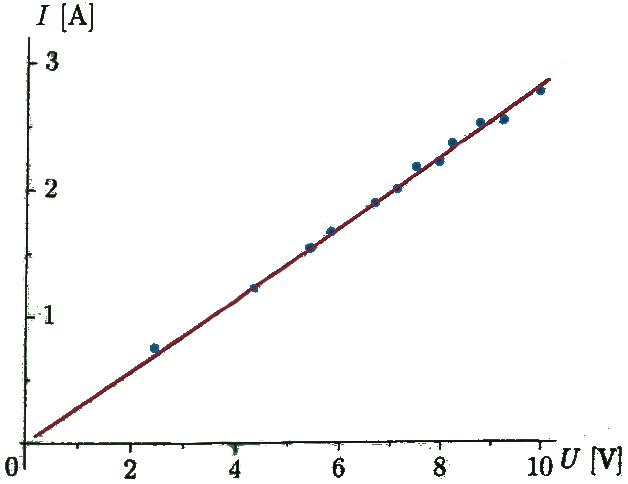
\includegraphics[width=0.8\linewidth]{mai_fig052.png}
  \captionof{figure}{Ověření Ohmová zákona lineární regresí.
  \cite[s.~263]{Musilova2009MA1}
  \label{mai:fig052}}
  \par}
  Pro odpor vychází \(R\doteq\SI{3.52}{\ohm}\). Součet čtverců odchylek přímky se směrnicí \(i/R
  = (1/\num{3.52})\Omega^{-1}\) od souboru bodů grafu je
  \begin{equation*}
    D(R) = \sum_{i=1}^{n}(U_i - R\cdot I_i)^2 \doteq\num{0.01},
  \end{equation*}
  \(\sigma(R) = \sqrt{D(R)/(n-1)}\doteq\sqrt{(\num{0.11}/11)}\doteq\num{0.03}\).  Graf přímky \(U
  = R\cdot I = \num{3.52}\cdot I\) proložené body je na obrázku \ref{mai:fig052}.
\end{mathexam}
      %---------------------------------------------------------------
      
      Popsaný způsob nalezení hodnoty elektrického odporu vodiče v příkladu \ref{mai:exam076} se
      nazývá\textbf{ metodou nejmenších čtverců} (minimalizuje součet čtverců odchylek prokládané
      závislosti od souboru naměřených bodů), v případě použití lineárního modelu, jako tomu bylo u
      Ohmová zákona, pak jde o \textbf{lineární regresi}
      
      Obdobně se postupuje, je-li některá z měřených veličin lineární funkcí veličin jiných s 
      neznámými koeficienty lineární kombinace. Nechť
      \begin{equation*}
        Z = f(X_1, X_2, \ldots, X_K) = A_1X_1 + A_2X_2 + \cdots + A_KX_K.
      \end{equation*}
      Předpokládejme, že veličiny \(X_1, X_2, \ldots, X_K\) a \(Z\) měříme \(n\)-krát a naměříme 
      hodnoty
      \begin{equation*}
        X_j = \lbrace x_{j1}, \ldots x_{jn} \rbrace, \; 1 \leq j \leq K, \; 
        Z = \lbrace z_{1}, \ldots z_{n} \rbrace
      \end{equation*}
      Součet čtverců odchylek teoretické závislosti od naměřených bodů je
      \begin{equation*}
        D(Z) = \sum_{i=1}^{n}\left(z_i - \sum_{j=1}^{K}A_jx_{ji}\right)^2.
      \end{equation*}
      Nutnou podmínkou pro minimum tohoto výrazu jakožto funkce proměnných \(A_x, A_2, \ldots, A_K\)
      je platnost souboru rovnic
      \begin{equation*}
        \pder{D(Z)}{A_p} = 0 \Rightarrow 
        \sum_{i=1}^{n}2\left(z_i - \sum_{j=1}^{K}A_jx_{ji}\right)\cdot x_{pi} = 0
      \end{equation*}
      pro \(1 \leq i \leq n, 1 \leq j \leq K\). Tyto podmínky představují nehomogenní soustavu 
      \(K\) rovnic pro \(K\) neznámých \(( A_1, A_2, \ldots, A_K)\). Rozšířená matice soustavy je
      \begin{strip}
      \begin{equation*}
        \overline{B} = (A\lvert B) = 
          \left(
            \begin{array}{cccc|c}
              \sum_{i=1}^{n}x_{1i}x_{1i} & \sum_{i=1}^{n}x_{1i}x_{2i} & \cdots & 
              \sum_{i=1}^{n}x_{1i}x_{Ki} & \sum_{i=1}^{n}z_{i}x_{1i}                    \\
              \sum_{i=1}^{n}x_{1i}x_{1i} & \sum_{i=1}^{n}x_{2i}x_{2i} & \cdots & 
              \sum_{i=1}^{n}x_{2i}x_{Ki} & \sum_{i=1}^{n}z_{i}x_{2i}                    \\
                        \cdots           & \cdots & \cdots & \cdots   & \cdots          \\
              \sum_{i=1}^{n}x_{Ki}x_{1i} & \sum_{i=1}^{n}x_{Ki}x_{2i} & \cdots & 
              \sum_{i=1}^{n}x_{Ki}x_{Ki} & \sum_{i=1}^{n}z_{i}x_{Ki}                    \\
            \end{array}
          \right),
      \end{equation*}
      \end{strip}
      \begin{equation*}
        \sigma(z) = \sqrt{\dfrac{D(z)}{n - K}}.
      \end{equation*}
      V dalších kapitolách věnovaných lineární algebře se k tomuto problému znovu vrátíme a ukážeme,
      že jej lze elegantně řešit také jako úlohu algebraickou, konkrétně úlohu o ortogonální
      projekci vektorů na podprostory.
      
%} %tikzset
%---------------------------------------------------------------------------------------------------
